% Created by tikzDevice version 0.9 on 2016-03-14 23:41:43
% !TEX encoding = UTF-8 Unicode
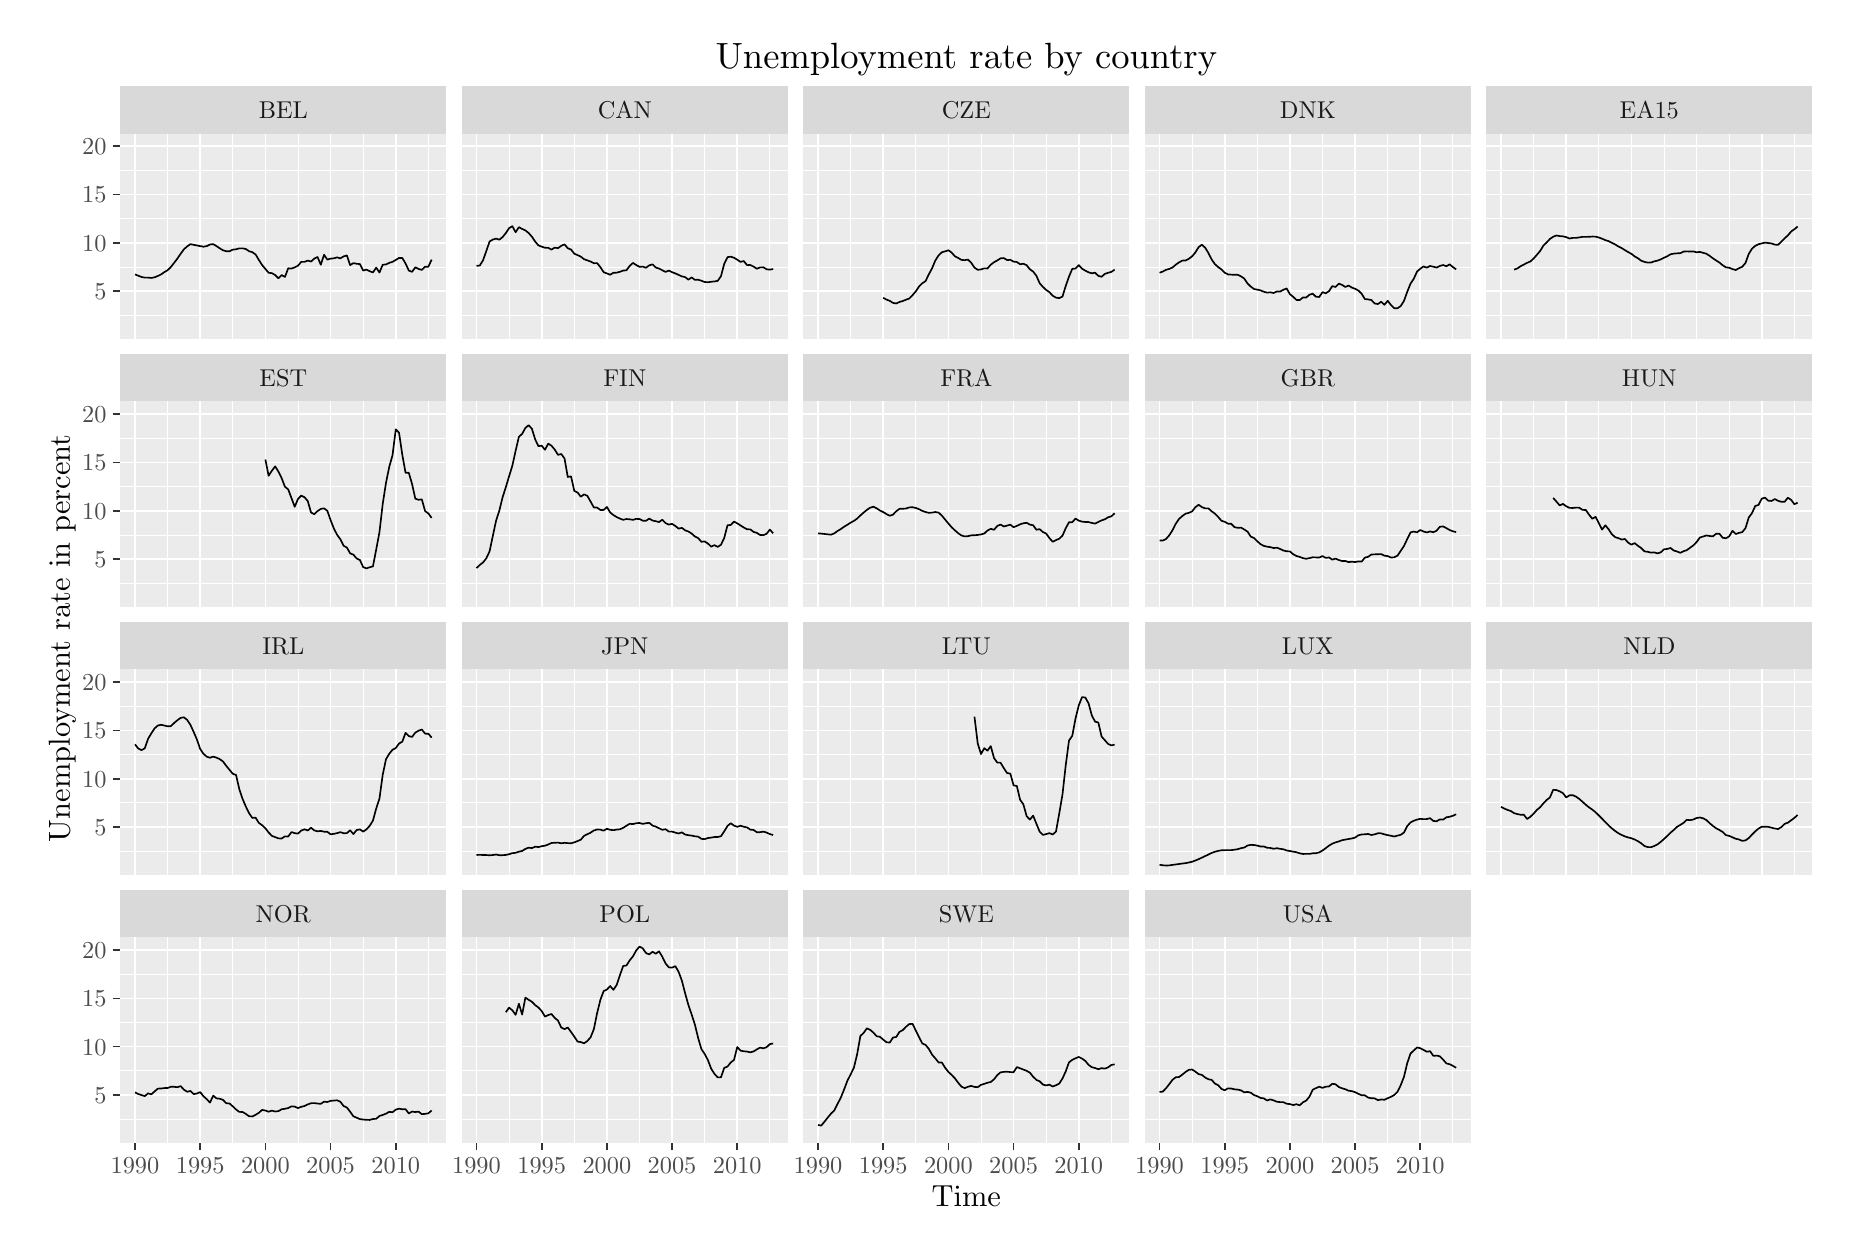
\begin{tikzpicture}[x=1pt,y=1pt]
\definecolor{fillColor}{RGB}{255,255,255}
\path[use as bounding box,fill=fillColor,fill opacity=0.00] (0,0) rectangle (650.43,433.62);
\begin{scope}
\path[clip] (  0.00,  0.00) rectangle (650.43,433.62);
\definecolor{drawColor}{RGB}{255,255,255}
\definecolor{fillColor}{RGB}{255,255,255}

\path[draw=drawColor,line width= 0.6pt,line join=round,line cap=round,fill=fillColor] (  0.00,  0.00) rectangle (650.43,433.62);
\end{scope}
\begin{scope}
\path[clip] ( 33.42,321.12) rectangle (151.33,395.37);
\definecolor{fillColor}{gray}{0.92}

\path[fill=fillColor] ( 33.42,321.12) rectangle (151.33,395.37);
\definecolor{drawColor}{RGB}{255,255,255}

\path[draw=drawColor,line width= 0.3pt,line join=round] ( 33.42,329.69) --
	(151.33,329.69);

\path[draw=drawColor,line width= 0.3pt,line join=round] ( 33.42,347.13) --
	(151.33,347.13);

\path[draw=drawColor,line width= 0.3pt,line join=round] ( 33.42,364.58) --
	(151.33,364.58);

\path[draw=drawColor,line width= 0.3pt,line join=round] ( 33.42,382.02) --
	(151.33,382.02);

\path[draw=drawColor,line width= 0.3pt,line join=round] ( 50.56,321.12) --
	( 50.56,395.37);

\path[draw=drawColor,line width= 0.3pt,line join=round] ( 74.12,321.12) --
	( 74.12,395.37);

\path[draw=drawColor,line width= 0.3pt,line join=round] ( 97.67,321.12) --
	( 97.67,395.37);

\path[draw=drawColor,line width= 0.3pt,line join=round] (121.23,321.12) --
	(121.23,395.37);

\path[draw=drawColor,line width= 0.3pt,line join=round] (144.79,321.12) --
	(144.79,395.37);

\path[draw=drawColor,line width= 0.6pt,line join=round] ( 33.42,338.41) --
	(151.33,338.41);

\path[draw=drawColor,line width= 0.6pt,line join=round] ( 33.42,355.85) --
	(151.33,355.85);

\path[draw=drawColor,line width= 0.6pt,line join=round] ( 33.42,373.30) --
	(151.33,373.30);

\path[draw=drawColor,line width= 0.6pt,line join=round] ( 33.42,390.74) --
	(151.33,390.74);

\path[draw=drawColor,line width= 0.6pt,line join=round] ( 38.78,321.12) --
	( 38.78,395.37);

\path[draw=drawColor,line width= 0.6pt,line join=round] ( 62.34,321.12) --
	( 62.34,395.37);

\path[draw=drawColor,line width= 0.6pt,line join=round] ( 85.90,321.12) --
	( 85.90,395.37);

\path[draw=drawColor,line width= 0.6pt,line join=round] (109.45,321.12) --
	(109.45,395.37);

\path[draw=drawColor,line width= 0.6pt,line join=round] (133.01,321.12) --
	(133.01,395.37);
\definecolor{drawColor}{RGB}{0,0,0}

\path[draw=drawColor,line width= 0.6pt,line join=round] ( 38.78,344.46) --
	( 39.96,343.99) --
	( 41.14,343.53) --
	( 42.32,343.29) --
	( 43.49,343.29) --
	( 44.67,343.18) --
	( 45.85,343.41) --
	( 47.03,343.88) --
	( 48.21,344.46) --
	( 49.38,345.27) --
	( 50.56,345.97) --
	( 51.74,347.13) --
	( 52.92,348.64) --
	( 54.09,350.16) --
	( 55.27,351.90) --
	( 56.45,353.53) --
	( 57.63,354.57) --
	( 58.81,355.39) --
	( 59.98,355.16) --
	( 61.16,354.92) --
	( 62.34,354.69) --
	( 63.52,354.46) --
	( 64.70,354.69) --
	( 65.87,355.27) --
	( 67.05,355.39) --
	( 68.23,354.69) --
	( 69.41,353.88) --
	( 70.58,353.18) --
	( 71.76,352.83) --
	( 72.94,352.83) --
	( 74.12,353.41) --
	( 75.30,353.53) --
	( 76.47,353.88) --
	( 77.65,353.88) --
	( 78.83,353.64) --
	( 80.01,352.83) --
	( 81.19,352.48) --
	( 82.36,351.67) --
	( 83.54,349.69) --
	( 84.72,347.83) --
	( 85.90,346.43) --
	( 87.07,345.04) --
	( 88.25,344.92) --
	( 89.43,344.22) --
	( 90.61,343.06) --
	( 91.79,344.22) --
	( 92.96,343.53) --
	( 94.14,346.67) --
	( 95.32,346.55) --
	( 96.50,347.02) --
	( 97.67,347.60) --
	( 98.85,348.99) --
	(100.03,348.99) --
	(101.21,349.46) --
	(102.39,349.11) --
	(103.56,350.16) --
	(104.74,350.74) --
	(105.92,347.95) --
	(107.10,351.55) --
	(108.28,349.81) --
	(109.45,350.16) --
	(110.63,350.27) --
	(111.81,350.62) --
	(112.99,350.27) --
	(114.16,350.97) --
	(115.34,351.32) --
	(116.52,347.83) --
	(117.70,348.53) --
	(118.88,348.30) --
	(120.05,348.18) --
	(121.23,345.85) --
	(122.41,346.20) --
	(123.59,345.62) --
	(124.76,345.16) --
	(125.94,346.90) --
	(127.12,345.16) --
	(128.30,347.95) --
	(129.48,348.06) --
	(130.65,348.64) --
	(131.83,348.99) --
	(133.01,349.69) --
	(134.19,350.39) --
	(135.37,350.39) --
	(136.54,348.41) --
	(137.72,345.85) --
	(138.90,345.39) --
	(140.08,347.02) --
	(141.25,346.43) --
	(142.43,346.09) --
	(143.61,347.25) --
	(144.79,347.25) --
	(145.97,349.81);
\end{scope}
\begin{scope}
\path[clip] (156.83,321.12) rectangle (274.73,395.37);
\definecolor{fillColor}{gray}{0.92}

\path[fill=fillColor] (156.83,321.12) rectangle (274.73,395.37);
\definecolor{drawColor}{RGB}{255,255,255}

\path[draw=drawColor,line width= 0.3pt,line join=round] (156.83,329.69) --
	(274.73,329.69);

\path[draw=drawColor,line width= 0.3pt,line join=round] (156.83,347.13) --
	(274.73,347.13);

\path[draw=drawColor,line width= 0.3pt,line join=round] (156.83,364.58) --
	(274.73,364.58);

\path[draw=drawColor,line width= 0.3pt,line join=round] (156.83,382.02) --
	(274.73,382.02);

\path[draw=drawColor,line width= 0.3pt,line join=round] (173.96,321.12) --
	(173.96,395.37);

\path[draw=drawColor,line width= 0.3pt,line join=round] (197.52,321.12) --
	(197.52,395.37);

\path[draw=drawColor,line width= 0.3pt,line join=round] (221.08,321.12) --
	(221.08,395.37);

\path[draw=drawColor,line width= 0.3pt,line join=round] (244.63,321.12) --
	(244.63,395.37);

\path[draw=drawColor,line width= 0.3pt,line join=round] (268.19,321.12) --
	(268.19,395.37);

\path[draw=drawColor,line width= 0.6pt,line join=round] (156.83,338.41) --
	(274.73,338.41);

\path[draw=drawColor,line width= 0.6pt,line join=round] (156.83,355.85) --
	(274.73,355.85);

\path[draw=drawColor,line width= 0.6pt,line join=round] (156.83,373.30) --
	(274.73,373.30);

\path[draw=drawColor,line width= 0.6pt,line join=round] (156.83,390.74) --
	(274.73,390.74);

\path[draw=drawColor,line width= 0.6pt,line join=round] (162.18,321.12) --
	(162.18,395.37);

\path[draw=drawColor,line width= 0.6pt,line join=round] (185.74,321.12) --
	(185.74,395.37);

\path[draw=drawColor,line width= 0.6pt,line join=round] (209.30,321.12) --
	(209.30,395.37);

\path[draw=drawColor,line width= 0.6pt,line join=round] (232.85,321.12) --
	(232.85,395.37);

\path[draw=drawColor,line width= 0.6pt,line join=round] (256.41,321.12) --
	(256.41,395.37);
\definecolor{drawColor}{RGB}{0,0,0}

\path[draw=drawColor,line width= 0.6pt,line join=round] (162.18,347.55) --
	(163.36,347.66) --
	(164.54,349.56) --
	(165.72,352.87) --
	(166.90,356.34) --
	(168.07,357.04) --
	(169.25,357.39) --
	(170.43,357.02) --
	(171.61,357.94) --
	(172.78,359.40) --
	(173.96,361.18) --
	(175.14,361.87) --
	(176.32,359.70) --
	(177.50,361.51) --
	(178.67,360.90) --
	(179.85,360.36) --
	(181.03,359.41) --
	(182.21,358.08) --
	(183.39,356.31) --
	(184.56,354.95) --
	(185.74,354.48) --
	(186.92,354.09) --
	(188.10,354.04) --
	(189.27,353.43) --
	(190.45,354.14) --
	(191.63,353.92) --
	(192.81,354.80) --
	(193.99,355.32) --
	(195.16,353.91) --
	(196.34,353.45) --
	(197.52,351.94) --
	(198.70,351.43) --
	(199.87,350.88) --
	(201.05,349.95) --
	(202.23,349.54) --
	(203.41,349.10) --
	(204.59,348.50) --
	(205.76,348.55) --
	(206.94,347.09) --
	(208.12,345.26) --
	(209.30,344.82) --
	(210.48,344.33) --
	(211.65,345.04) --
	(212.83,345.09) --
	(214.01,345.41) --
	(215.19,345.84) --
	(216.36,345.95) --
	(217.54,347.53) --
	(218.72,348.61) --
	(219.90,347.84) --
	(221.08,347.20) --
	(222.25,347.28) --
	(223.43,346.86) --
	(224.61,347.74) --
	(225.79,348.08) --
	(226.97,346.96) --
	(228.14,346.57) --
	(229.32,345.97) --
	(230.50,345.37) --
	(231.68,345.84) --
	(232.85,345.25) --
	(234.03,344.82) --
	(235.21,344.29) --
	(236.39,343.74) --
	(237.57,343.49) --
	(238.74,342.56) --
	(239.92,343.37) --
	(241.10,342.48) --
	(242.28,342.54) --
	(243.45,342.17) --
	(244.63,341.71) --
	(245.81,341.64) --
	(246.99,341.80) --
	(248.17,341.92) --
	(249.34,342.12) --
	(250.52,343.80) --
	(251.70,348.30) --
	(252.88,350.69) --
	(254.06,350.86) --
	(255.23,350.49) --
	(256.41,349.76) --
	(257.59,348.97) --
	(258.77,349.29) --
	(259.94,347.81) --
	(261.12,347.86) --
	(262.30,347.28) --
	(263.48,346.50) --
	(264.66,346.99) --
	(265.83,347.02) --
	(267.01,346.31) --
	(268.19,346.19) --
	(269.37,346.39);
\end{scope}
\begin{scope}
\path[clip] (280.23,321.12) rectangle (398.13,395.37);
\definecolor{fillColor}{gray}{0.92}

\path[fill=fillColor] (280.23,321.12) rectangle (398.13,395.37);
\definecolor{drawColor}{RGB}{255,255,255}

\path[draw=drawColor,line width= 0.3pt,line join=round] (280.23,329.69) --
	(398.13,329.69);

\path[draw=drawColor,line width= 0.3pt,line join=round] (280.23,347.13) --
	(398.13,347.13);

\path[draw=drawColor,line width= 0.3pt,line join=round] (280.23,364.58) --
	(398.13,364.58);

\path[draw=drawColor,line width= 0.3pt,line join=round] (280.23,382.02) --
	(398.13,382.02);

\path[draw=drawColor,line width= 0.3pt,line join=round] (297.36,321.12) --
	(297.36,395.37);

\path[draw=drawColor,line width= 0.3pt,line join=round] (320.92,321.12) --
	(320.92,395.37);

\path[draw=drawColor,line width= 0.3pt,line join=round] (344.48,321.12) --
	(344.48,395.37);

\path[draw=drawColor,line width= 0.3pt,line join=round] (368.03,321.12) --
	(368.03,395.37);

\path[draw=drawColor,line width= 0.3pt,line join=round] (391.59,321.12) --
	(391.59,395.37);

\path[draw=drawColor,line width= 0.6pt,line join=round] (280.23,338.41) --
	(398.13,338.41);

\path[draw=drawColor,line width= 0.6pt,line join=round] (280.23,355.85) --
	(398.13,355.85);

\path[draw=drawColor,line width= 0.6pt,line join=round] (280.23,373.30) --
	(398.13,373.30);

\path[draw=drawColor,line width= 0.6pt,line join=round] (280.23,390.74) --
	(398.13,390.74);

\path[draw=drawColor,line width= 0.6pt,line join=round] (285.59,321.12) --
	(285.59,395.37);

\path[draw=drawColor,line width= 0.6pt,line join=round] (309.14,321.12) --
	(309.14,395.37);

\path[draw=drawColor,line width= 0.6pt,line join=round] (332.70,321.12) --
	(332.70,395.37);

\path[draw=drawColor,line width= 0.6pt,line join=round] (356.26,321.12) --
	(356.26,395.37);

\path[draw=drawColor,line width= 0.6pt,line join=round] (379.81,321.12) --
	(379.81,395.37);
\definecolor{drawColor}{RGB}{0,0,0}

\path[draw=drawColor,line width= 0.6pt,line join=round] (309.14,335.99) --
	(310.32,335.37) --
	(311.50,334.91) --
	(312.68,334.16) --
	(313.85,333.96) --
	(315.03,334.50) --
	(316.21,334.84) --
	(317.39,335.32) --
	(318.56,335.73) --
	(319.74,336.96) --
	(320.92,338.33) --
	(322.10,340.09) --
	(323.28,341.27) --
	(324.45,342.05) --
	(325.63,344.49) --
	(326.81,346.68) --
	(327.99,349.52) --
	(329.17,351.35) --
	(330.34,352.46) --
	(331.52,352.79) --
	(332.70,353.19) --
	(333.88,352.34) --
	(335.05,351.01) --
	(336.23,350.40) --
	(337.41,349.71) --
	(338.59,349.60) --
	(339.77,349.81) --
	(340.94,348.67) --
	(342.12,346.91) --
	(343.30,346.12) --
	(344.48,346.26) --
	(345.66,346.64) --
	(346.83,346.61) --
	(348.01,347.98) --
	(349.19,348.86) --
	(350.37,349.51) --
	(351.54,350.26) --
	(352.72,350.36) --
	(353.90,349.64) --
	(355.08,349.73) --
	(356.26,349.07) --
	(357.43,348.95) --
	(358.61,348.14) --
	(359.79,348.30) --
	(360.97,347.79) --
	(362.14,346.30) --
	(363.32,345.49) --
	(364.50,343.95) --
	(365.68,341.26) --
	(366.86,339.94) --
	(368.03,338.85) --
	(369.21,338.03) --
	(370.39,336.76) --
	(371.57,336.07) --
	(372.75,335.89) --
	(373.92,336.44) --
	(375.10,340.30) --
	(376.28,343.65) --
	(377.46,346.48) --
	(378.63,346.56) --
	(379.81,347.82) --
	(380.99,346.53) --
	(382.17,345.81) --
	(383.35,345.23) --
	(384.52,344.86) --
	(385.70,345.08) --
	(386.88,343.92) --
	(388.06,343.61) --
	(389.23,344.65) --
	(390.41,345.03) --
	(391.59,345.38) --
	(392.77,346.18);
\end{scope}
\begin{scope}
\path[clip] (403.63,321.12) rectangle (521.53,395.37);
\definecolor{fillColor}{gray}{0.92}

\path[fill=fillColor] (403.63,321.12) rectangle (521.53,395.37);
\definecolor{drawColor}{RGB}{255,255,255}

\path[draw=drawColor,line width= 0.3pt,line join=round] (403.63,329.69) --
	(521.53,329.69);

\path[draw=drawColor,line width= 0.3pt,line join=round] (403.63,347.13) --
	(521.53,347.13);

\path[draw=drawColor,line width= 0.3pt,line join=round] (403.63,364.58) --
	(521.53,364.58);

\path[draw=drawColor,line width= 0.3pt,line join=round] (403.63,382.02) --
	(521.53,382.02);

\path[draw=drawColor,line width= 0.3pt,line join=round] (420.77,321.12) --
	(420.77,395.37);

\path[draw=drawColor,line width= 0.3pt,line join=round] (444.32,321.12) --
	(444.32,395.37);

\path[draw=drawColor,line width= 0.3pt,line join=round] (467.88,321.12) --
	(467.88,395.37);

\path[draw=drawColor,line width= 0.3pt,line join=round] (491.44,321.12) --
	(491.44,395.37);

\path[draw=drawColor,line width= 0.3pt,line join=round] (514.99,321.12) --
	(514.99,395.37);

\path[draw=drawColor,line width= 0.6pt,line join=round] (403.63,338.41) --
	(521.53,338.41);

\path[draw=drawColor,line width= 0.6pt,line join=round] (403.63,355.85) --
	(521.53,355.85);

\path[draw=drawColor,line width= 0.6pt,line join=round] (403.63,373.30) --
	(521.53,373.30);

\path[draw=drawColor,line width= 0.6pt,line join=round] (403.63,390.74) --
	(521.53,390.74);

\path[draw=drawColor,line width= 0.6pt,line join=round] (408.99,321.12) --
	(408.99,395.37);

\path[draw=drawColor,line width= 0.6pt,line join=round] (432.54,321.12) --
	(432.54,395.37);

\path[draw=drawColor,line width= 0.6pt,line join=round] (456.10,321.12) --
	(456.10,395.37);

\path[draw=drawColor,line width= 0.6pt,line join=round] (479.66,321.12) --
	(479.66,395.37);

\path[draw=drawColor,line width= 0.6pt,line join=round] (503.21,321.12) --
	(503.21,395.37);
\definecolor{drawColor}{RGB}{0,0,0}

\path[draw=drawColor,line width= 0.6pt,line join=round] (408.99,345.07) --
	(410.16,345.48) --
	(411.34,346.11) --
	(412.52,346.45) --
	(413.70,346.97) --
	(414.88,347.99) --
	(416.05,348.82) --
	(417.23,349.45) --
	(418.41,349.50) --
	(419.59,350.11) --
	(420.77,351.00) --
	(421.94,352.39) --
	(423.12,354.32) --
	(424.30,355.18) --
	(425.48,354.10) --
	(426.65,352.20) --
	(427.83,349.86) --
	(429.01,348.16) --
	(430.19,347.11) --
	(431.37,346.24) --
	(432.54,345.07) --
	(433.72,344.45) --
	(434.90,344.38) --
	(436.08,344.30) --
	(437.25,344.34) --
	(438.43,343.76) --
	(439.61,342.94) --
	(440.79,341.18) --
	(441.97,340.05) --
	(443.14,339.17) --
	(444.32,338.96) --
	(445.50,338.69) --
	(446.68,338.20) --
	(447.86,337.86) --
	(449.03,337.99) --
	(450.21,337.74) --
	(451.39,338.31) --
	(452.57,338.27) --
	(453.74,338.91) --
	(454.92,339.38) --
	(456.10,337.32) --
	(457.28,336.36) --
	(458.46,335.24) --
	(459.63,335.18) --
	(460.81,336.12) --
	(461.99,336.12) --
	(463.17,337.12) --
	(464.34,337.49) --
	(465.52,336.37) --
	(466.70,336.31) --
	(467.88,338.03) --
	(469.06,337.63) --
	(470.23,338.40) --
	(471.41,340.23) --
	(472.59,339.91) --
	(473.77,341.12) --
	(474.95,340.68) --
	(476.12,339.91) --
	(477.30,340.43) --
	(478.48,339.71) --
	(479.66,339.25) --
	(480.83,338.64) --
	(482.01,337.50) --
	(483.19,335.54) --
	(484.37,335.43) --
	(485.55,335.20) --
	(486.72,333.95) --
	(487.90,333.75) --
	(489.08,334.58) --
	(490.26,333.48) --
	(491.44,334.92) --
	(492.61,333.40) --
	(493.79,332.22) --
	(494.97,332.22) --
	(496.15,333.02) --
	(497.32,334.89) --
	(498.50,338.15) --
	(499.68,341.10) --
	(500.86,342.87) --
	(502.04,345.49) --
	(503.21,346.50) --
	(504.39,347.34) --
	(505.57,346.90) --
	(506.75,347.50) --
	(507.92,347.24) --
	(509.10,346.94) --
	(510.28,347.51) --
	(511.46,347.85) --
	(512.64,347.40) --
	(513.81,348.10) --
	(514.99,347.12) --
	(516.17,346.28);
\end{scope}
\begin{scope}
\path[clip] (527.03,321.12) rectangle (644.93,395.37);
\definecolor{fillColor}{gray}{0.92}

\path[fill=fillColor] (527.03,321.12) rectangle (644.93,395.37);
\definecolor{drawColor}{RGB}{255,255,255}

\path[draw=drawColor,line width= 0.3pt,line join=round] (527.03,329.69) --
	(644.93,329.69);

\path[draw=drawColor,line width= 0.3pt,line join=round] (527.03,347.13) --
	(644.93,347.13);

\path[draw=drawColor,line width= 0.3pt,line join=round] (527.03,364.58) --
	(644.93,364.58);

\path[draw=drawColor,line width= 0.3pt,line join=round] (527.03,382.02) --
	(644.93,382.02);

\path[draw=drawColor,line width= 0.3pt,line join=round] (544.17,321.12) --
	(544.17,395.37);

\path[draw=drawColor,line width= 0.3pt,line join=round] (567.72,321.12) --
	(567.72,395.37);

\path[draw=drawColor,line width= 0.3pt,line join=round] (591.28,321.12) --
	(591.28,395.37);

\path[draw=drawColor,line width= 0.3pt,line join=round] (614.84,321.12) --
	(614.84,395.37);

\path[draw=drawColor,line width= 0.3pt,line join=round] (638.39,321.12) --
	(638.39,395.37);

\path[draw=drawColor,line width= 0.6pt,line join=round] (527.03,338.41) --
	(644.93,338.41);

\path[draw=drawColor,line width= 0.6pt,line join=round] (527.03,355.85) --
	(644.93,355.85);

\path[draw=drawColor,line width= 0.6pt,line join=round] (527.03,373.30) --
	(644.93,373.30);

\path[draw=drawColor,line width= 0.6pt,line join=round] (527.03,390.74) --
	(644.93,390.74);

\path[draw=drawColor,line width= 0.6pt,line join=round] (532.39,321.12) --
	(532.39,395.37);

\path[draw=drawColor,line width= 0.6pt,line join=round] (555.94,321.12) --
	(555.94,395.37);

\path[draw=drawColor,line width= 0.6pt,line join=round] (579.50,321.12) --
	(579.50,395.37);

\path[draw=drawColor,line width= 0.6pt,line join=round] (603.06,321.12) --
	(603.06,395.37);

\path[draw=drawColor,line width= 0.6pt,line join=round] (626.61,321.12) --
	(626.61,395.37);
\definecolor{drawColor}{RGB}{0,0,0}

\path[draw=drawColor,line width= 0.6pt,line join=round] (537.10,346.18) --
	(538.28,346.60) --
	(539.45,347.41) --
	(540.63,348.02) --
	(541.81,348.64) --
	(542.99,349.14) --
	(544.17,350.20) --
	(545.34,351.53) --
	(546.52,352.92) --
	(547.70,354.87) --
	(548.88,356.01) --
	(550.06,357.27) --
	(551.23,358.07) --
	(552.41,358.52) --
	(553.59,358.30) --
	(554.77,358.21) --
	(555.94,357.93) --
	(557.12,357.43) --
	(558.30,357.65) --
	(559.48,357.65) --
	(560.66,357.83) --
	(561.83,358.03) --
	(563.01,358.02) --
	(564.19,358.05) --
	(565.37,358.13) --
	(566.55,358.11) --
	(567.72,357.78) --
	(568.90,357.37) --
	(570.08,356.85) --
	(571.26,356.48) --
	(572.43,355.87) --
	(573.61,355.30) --
	(574.79,354.55) --
	(575.97,353.98) --
	(577.15,353.23) --
	(578.32,352.53) --
	(579.50,351.90) --
	(580.68,350.96) --
	(581.86,350.29) --
	(583.03,349.41) --
	(584.21,348.99) --
	(585.39,348.72) --
	(586.57,348.75) --
	(587.75,349.17) --
	(588.92,349.43) --
	(590.10,349.89) --
	(591.28,350.47) --
	(592.46,351.01) --
	(593.64,351.73) --
	(594.81,351.96) --
	(595.99,352.07) --
	(597.17,352.12) --
	(598.35,352.71) --
	(599.52,352.78) --
	(600.70,352.74) --
	(601.88,352.76) --
	(603.06,352.46) --
	(604.24,352.59) --
	(605.41,352.26) --
	(606.59,351.94) --
	(607.77,351.17) --
	(608.95,350.27) --
	(610.12,349.48) --
	(611.30,348.75) --
	(612.48,347.76) --
	(613.66,347.01) --
	(614.84,346.87) --
	(616.01,346.39) --
	(617.19,346.04) --
	(618.37,346.70) --
	(619.55,347.22) --
	(620.73,348.59) --
	(621.90,351.85) --
	(623.08,353.76) --
	(624.26,354.79) --
	(625.44,355.38) --
	(626.61,355.65) --
	(627.79,355.95) --
	(628.97,355.79) --
	(630.15,355.64) --
	(631.33,355.22) --
	(632.50,355.15) --
	(633.68,356.30) --
	(634.86,357.50) --
	(636.04,358.55) --
	(637.22,359.96) --
	(638.39,360.78) --
	(639.57,361.75);
\end{scope}
\begin{scope}
\path[clip] ( 33.42,224.31) rectangle (151.33,298.56);
\definecolor{fillColor}{gray}{0.92}

\path[fill=fillColor] ( 33.42,224.31) rectangle (151.33,298.56);
\definecolor{drawColor}{RGB}{255,255,255}

\path[draw=drawColor,line width= 0.3pt,line join=round] ( 33.42,232.88) --
	(151.33,232.88);

\path[draw=drawColor,line width= 0.3pt,line join=round] ( 33.42,250.32) --
	(151.33,250.32);

\path[draw=drawColor,line width= 0.3pt,line join=round] ( 33.42,267.77) --
	(151.33,267.77);

\path[draw=drawColor,line width= 0.3pt,line join=round] ( 33.42,285.21) --
	(151.33,285.21);

\path[draw=drawColor,line width= 0.3pt,line join=round] ( 50.56,224.31) --
	( 50.56,298.56);

\path[draw=drawColor,line width= 0.3pt,line join=round] ( 74.12,224.31) --
	( 74.12,298.56);

\path[draw=drawColor,line width= 0.3pt,line join=round] ( 97.67,224.31) --
	( 97.67,298.56);

\path[draw=drawColor,line width= 0.3pt,line join=round] (121.23,224.31) --
	(121.23,298.56);

\path[draw=drawColor,line width= 0.3pt,line join=round] (144.79,224.31) --
	(144.79,298.56);

\path[draw=drawColor,line width= 0.6pt,line join=round] ( 33.42,241.60) --
	(151.33,241.60);

\path[draw=drawColor,line width= 0.6pt,line join=round] ( 33.42,259.04) --
	(151.33,259.04);

\path[draw=drawColor,line width= 0.6pt,line join=round] ( 33.42,276.49) --
	(151.33,276.49);

\path[draw=drawColor,line width= 0.6pt,line join=round] ( 33.42,293.93) --
	(151.33,293.93);

\path[draw=drawColor,line width= 0.6pt,line join=round] ( 38.78,224.31) --
	( 38.78,298.56);

\path[draw=drawColor,line width= 0.6pt,line join=round] ( 62.34,224.31) --
	( 62.34,298.56);

\path[draw=drawColor,line width= 0.6pt,line join=round] ( 85.90,224.31) --
	( 85.90,298.56);

\path[draw=drawColor,line width= 0.6pt,line join=round] (109.45,224.31) --
	(109.45,298.56);

\path[draw=drawColor,line width= 0.6pt,line join=round] (133.01,224.31) --
	(133.01,298.56);
\definecolor{drawColor}{RGB}{0,0,0}

\path[draw=drawColor,line width= 0.6pt,line join=round] ( 85.90,277.56) --
	( 87.07,271.72) --
	( 88.25,273.53) --
	( 89.43,275.09) --
	( 90.61,273.20) --
	( 91.79,270.80) --
	( 92.96,267.73) --
	( 94.14,266.78) --
	( 95.32,263.63) --
	( 96.50,260.50) --
	( 97.67,263.30) --
	( 98.85,264.54) --
	(100.03,263.95) --
	(101.21,262.56) --
	(102.39,258.43) --
	(103.56,257.83) --
	(104.74,258.94) --
	(105.92,259.72) --
	(107.10,259.93) --
	(108.28,259.04) --
	(109.45,255.70) --
	(110.63,252.69) --
	(111.81,250.36) --
	(112.99,248.76) --
	(114.16,246.38) --
	(115.34,245.77) --
	(116.52,243.68) --
	(117.70,243.18) --
	(118.88,241.79) --
	(120.05,241.26) --
	(121.23,238.69) --
	(122.41,238.22) --
	(123.59,238.63) --
	(124.76,238.97) --
	(125.94,245.03) --
	(127.12,251.35) --
	(128.30,261.55) --
	(129.48,269.15) --
	(130.65,274.91) --
	(131.83,279.09) --
	(133.01,288.47) --
	(134.19,287.25) --
	(135.37,279.29) --
	(136.54,272.79) --
	(137.72,272.77) --
	(138.90,268.71) --
	(140.08,263.40) --
	(141.25,263.03) --
	(142.43,263.16) --
	(143.61,258.92) --
	(144.79,258.08) --
	(145.97,256.46);
\end{scope}
\begin{scope}
\path[clip] (156.83,224.31) rectangle (274.73,298.56);
\definecolor{fillColor}{gray}{0.92}

\path[fill=fillColor] (156.83,224.31) rectangle (274.73,298.56);
\definecolor{drawColor}{RGB}{255,255,255}

\path[draw=drawColor,line width= 0.3pt,line join=round] (156.83,232.88) --
	(274.73,232.88);

\path[draw=drawColor,line width= 0.3pt,line join=round] (156.83,250.32) --
	(274.73,250.32);

\path[draw=drawColor,line width= 0.3pt,line join=round] (156.83,267.77) --
	(274.73,267.77);

\path[draw=drawColor,line width= 0.3pt,line join=round] (156.83,285.21) --
	(274.73,285.21);

\path[draw=drawColor,line width= 0.3pt,line join=round] (173.96,224.31) --
	(173.96,298.56);

\path[draw=drawColor,line width= 0.3pt,line join=round] (197.52,224.31) --
	(197.52,298.56);

\path[draw=drawColor,line width= 0.3pt,line join=round] (221.08,224.31) --
	(221.08,298.56);

\path[draw=drawColor,line width= 0.3pt,line join=round] (244.63,224.31) --
	(244.63,298.56);

\path[draw=drawColor,line width= 0.3pt,line join=round] (268.19,224.31) --
	(268.19,298.56);

\path[draw=drawColor,line width= 0.6pt,line join=round] (156.83,241.60) --
	(274.73,241.60);

\path[draw=drawColor,line width= 0.6pt,line join=round] (156.83,259.04) --
	(274.73,259.04);

\path[draw=drawColor,line width= 0.6pt,line join=round] (156.83,276.49) --
	(274.73,276.49);

\path[draw=drawColor,line width= 0.6pt,line join=round] (156.83,293.93) --
	(274.73,293.93);

\path[draw=drawColor,line width= 0.6pt,line join=round] (162.18,224.31) --
	(162.18,298.56);

\path[draw=drawColor,line width= 0.6pt,line join=round] (185.74,224.31) --
	(185.74,298.56);

\path[draw=drawColor,line width= 0.6pt,line join=round] (209.30,224.31) --
	(209.30,298.56);

\path[draw=drawColor,line width= 0.6pt,line join=round] (232.85,224.31) --
	(232.85,298.56);

\path[draw=drawColor,line width= 0.6pt,line join=round] (256.41,224.31) --
	(256.41,298.56);
\definecolor{drawColor}{RGB}{0,0,0}

\path[draw=drawColor,line width= 0.6pt,line join=round] (162.18,238.35) --
	(163.36,239.46) --
	(164.54,240.37) --
	(165.72,241.86) --
	(166.90,244.36) --
	(168.07,249.89) --
	(169.25,255.44) --
	(170.43,259.10) --
	(171.61,263.92) --
	(172.78,267.59) --
	(173.96,271.52) --
	(175.14,275.36) --
	(176.32,280.71) --
	(177.50,285.79) --
	(178.67,286.84) --
	(179.85,288.99) --
	(181.03,289.98) --
	(182.21,288.66) --
	(183.39,284.81) --
	(184.56,282.41) --
	(185.74,282.55) --
	(186.92,281.09) --
	(188.10,283.30) --
	(189.27,282.57) --
	(190.45,281.16) --
	(191.63,279.26) --
	(192.81,279.56) --
	(193.99,277.95) --
	(195.16,271.26) --
	(196.34,271.49) --
	(197.52,266.21) --
	(198.70,265.65) --
	(199.87,264.14) --
	(201.05,264.96) --
	(202.23,264.46) --
	(203.41,262.37) --
	(204.59,260.23) --
	(205.76,260.21) --
	(206.94,259.33) --
	(208.12,259.35) --
	(209.30,260.42) --
	(210.48,258.44) --
	(211.65,257.50) --
	(212.83,256.77) --
	(214.01,256.22) --
	(215.19,255.77) --
	(216.36,256.07) --
	(217.54,255.97) --
	(218.72,255.76) --
	(219.90,256.12) --
	(221.08,256.06) --
	(222.25,255.47) --
	(223.43,255.42) --
	(224.61,256.21) --
	(225.79,255.53) --
	(226.97,255.28) --
	(228.14,254.97) --
	(229.32,255.82) --
	(230.50,254.58) --
	(231.68,254.05) --
	(232.85,254.33) --
	(234.03,253.56) --
	(235.21,252.60) --
	(236.39,252.88) --
	(237.57,251.98) --
	(238.74,251.56) --
	(239.92,250.82) --
	(241.10,249.75) --
	(242.28,249.18) --
	(243.45,247.84) --
	(244.63,247.98) --
	(245.81,247.20) --
	(246.99,246.09) --
	(248.17,246.63) --
	(249.34,246.00) --
	(250.52,246.76) --
	(251.70,249.24) --
	(252.88,253.80) --
	(254.06,253.93) --
	(255.23,255.13) --
	(256.41,254.50) --
	(257.59,253.74) --
	(258.77,253.00) --
	(259.94,252.36) --
	(261.12,252.33) --
	(262.30,251.41) --
	(263.48,251.07) --
	(264.66,250.30) --
	(265.83,250.25) --
	(267.01,250.73) --
	(268.19,252.26) --
	(269.37,250.92);
\end{scope}
\begin{scope}
\path[clip] (280.23,224.31) rectangle (398.13,298.56);
\definecolor{fillColor}{gray}{0.92}

\path[fill=fillColor] (280.23,224.31) rectangle (398.13,298.56);
\definecolor{drawColor}{RGB}{255,255,255}

\path[draw=drawColor,line width= 0.3pt,line join=round] (280.23,232.88) --
	(398.13,232.88);

\path[draw=drawColor,line width= 0.3pt,line join=round] (280.23,250.32) --
	(398.13,250.32);

\path[draw=drawColor,line width= 0.3pt,line join=round] (280.23,267.77) --
	(398.13,267.77);

\path[draw=drawColor,line width= 0.3pt,line join=round] (280.23,285.21) --
	(398.13,285.21);

\path[draw=drawColor,line width= 0.3pt,line join=round] (297.36,224.31) --
	(297.36,298.56);

\path[draw=drawColor,line width= 0.3pt,line join=round] (320.92,224.31) --
	(320.92,298.56);

\path[draw=drawColor,line width= 0.3pt,line join=round] (344.48,224.31) --
	(344.48,298.56);

\path[draw=drawColor,line width= 0.3pt,line join=round] (368.03,224.31) --
	(368.03,298.56);

\path[draw=drawColor,line width= 0.3pt,line join=round] (391.59,224.31) --
	(391.59,298.56);

\path[draw=drawColor,line width= 0.6pt,line join=round] (280.23,241.60) --
	(398.13,241.60);

\path[draw=drawColor,line width= 0.6pt,line join=round] (280.23,259.04) --
	(398.13,259.04);

\path[draw=drawColor,line width= 0.6pt,line join=round] (280.23,276.49) --
	(398.13,276.49);

\path[draw=drawColor,line width= 0.6pt,line join=round] (280.23,293.93) --
	(398.13,293.93);

\path[draw=drawColor,line width= 0.6pt,line join=round] (285.59,224.31) --
	(285.59,298.56);

\path[draw=drawColor,line width= 0.6pt,line join=round] (309.14,224.31) --
	(309.14,298.56);

\path[draw=drawColor,line width= 0.6pt,line join=round] (332.70,224.31) --
	(332.70,298.56);

\path[draw=drawColor,line width= 0.6pt,line join=round] (356.26,224.31) --
	(356.26,298.56);

\path[draw=drawColor,line width= 0.6pt,line join=round] (379.81,224.31) --
	(379.81,298.56);
\definecolor{drawColor}{RGB}{0,0,0}

\path[draw=drawColor,line width= 0.6pt,line join=round] (285.59,250.89) --
	(286.76,250.79) --
	(287.94,250.66) --
	(289.12,250.53) --
	(290.30,250.41) --
	(291.47,250.89) --
	(292.65,251.75) --
	(293.83,252.44) --
	(295.01,253.28) --
	(296.19,254.00) --
	(297.36,254.75) --
	(298.54,255.38) --
	(299.72,256.23) --
	(300.90,257.36) --
	(302.08,258.42) --
	(303.25,259.36) --
	(304.43,260.18) --
	(305.61,260.50) --
	(306.79,259.95) --
	(307.96,259.13) --
	(309.14,258.58) --
	(310.32,257.86) --
	(311.50,257.26) --
	(312.68,257.65) --
	(313.85,258.88) --
	(315.03,259.75) --
	(316.21,259.77) --
	(317.39,259.86) --
	(318.56,260.26) --
	(319.74,260.33) --
	(320.92,260.07) --
	(322.10,259.61) --
	(323.28,259.01) --
	(324.45,258.60) --
	(325.63,258.30) --
	(326.81,258.39) --
	(327.99,258.60) --
	(329.17,258.39) --
	(330.34,257.29) --
	(331.52,255.87) --
	(332.70,254.45) --
	(333.88,253.08) --
	(335.05,251.98) --
	(336.23,250.95) --
	(337.41,250.13) --
	(338.59,249.79) --
	(339.77,249.87) --
	(340.94,250.17) --
	(342.12,250.21) --
	(343.30,250.32) --
	(344.48,250.50) --
	(345.66,250.82) --
	(346.83,251.92) --
	(348.01,252.54) --
	(349.19,252.18) --
	(350.37,253.56) --
	(351.54,254.08) --
	(352.72,253.37) --
	(353.90,253.69) --
	(355.08,254.02) --
	(356.26,253.11) --
	(357.43,253.58) --
	(358.61,254.16) --
	(359.79,254.53) --
	(360.97,254.70) --
	(362.14,254.06) --
	(363.32,253.81) --
	(364.50,252.20) --
	(365.68,252.40) --
	(366.86,251.35) --
	(368.03,250.82) --
	(369.21,249.16) --
	(370.39,247.85) --
	(371.57,248.46) --
	(372.75,248.95) --
	(373.92,250.05) --
	(375.10,252.75) --
	(376.28,254.90) --
	(377.46,254.91) --
	(378.63,256.22) --
	(379.81,255.49) --
	(380.99,255.12) --
	(382.17,255.00) --
	(383.35,254.97) --
	(384.52,254.65) --
	(385.70,254.42) --
	(386.88,255.01) --
	(388.06,255.57) --
	(389.23,255.96) --
	(390.41,256.70) --
	(391.59,257.05) --
	(392.77,258.14);
\end{scope}
\begin{scope}
\path[clip] (403.63,224.31) rectangle (521.53,298.56);
\definecolor{fillColor}{gray}{0.92}

\path[fill=fillColor] (403.63,224.31) rectangle (521.53,298.56);
\definecolor{drawColor}{RGB}{255,255,255}

\path[draw=drawColor,line width= 0.3pt,line join=round] (403.63,232.88) --
	(521.53,232.88);

\path[draw=drawColor,line width= 0.3pt,line join=round] (403.63,250.32) --
	(521.53,250.32);

\path[draw=drawColor,line width= 0.3pt,line join=round] (403.63,267.77) --
	(521.53,267.77);

\path[draw=drawColor,line width= 0.3pt,line join=round] (403.63,285.21) --
	(521.53,285.21);

\path[draw=drawColor,line width= 0.3pt,line join=round] (420.77,224.31) --
	(420.77,298.56);

\path[draw=drawColor,line width= 0.3pt,line join=round] (444.32,224.31) --
	(444.32,298.56);

\path[draw=drawColor,line width= 0.3pt,line join=round] (467.88,224.31) --
	(467.88,298.56);

\path[draw=drawColor,line width= 0.3pt,line join=round] (491.44,224.31) --
	(491.44,298.56);

\path[draw=drawColor,line width= 0.3pt,line join=round] (514.99,224.31) --
	(514.99,298.56);

\path[draw=drawColor,line width= 0.6pt,line join=round] (403.63,241.60) --
	(521.53,241.60);

\path[draw=drawColor,line width= 0.6pt,line join=round] (403.63,259.04) --
	(521.53,259.04);

\path[draw=drawColor,line width= 0.6pt,line join=round] (403.63,276.49) --
	(521.53,276.49);

\path[draw=drawColor,line width= 0.6pt,line join=round] (403.63,293.93) --
	(521.53,293.93);

\path[draw=drawColor,line width= 0.6pt,line join=round] (408.99,224.31) --
	(408.99,298.56);

\path[draw=drawColor,line width= 0.6pt,line join=round] (432.54,224.31) --
	(432.54,298.56);

\path[draw=drawColor,line width= 0.6pt,line join=round] (456.10,224.31) --
	(456.10,298.56);

\path[draw=drawColor,line width= 0.6pt,line join=round] (479.66,224.31) --
	(479.66,298.56);

\path[draw=drawColor,line width= 0.6pt,line join=round] (503.21,224.31) --
	(503.21,298.56);
\definecolor{drawColor}{RGB}{0,0,0}

\path[draw=drawColor,line width= 0.6pt,line join=round] (408.99,248.34) --
	(410.16,248.29) --
	(411.34,248.85) --
	(412.52,250.20) --
	(413.70,252.06) --
	(414.88,254.38) --
	(416.05,256.11) --
	(417.23,257.15) --
	(418.41,258.00) --
	(419.59,258.30) --
	(420.77,258.83) --
	(421.94,260.33) --
	(423.12,261.21) --
	(424.30,260.39) --
	(425.48,259.90) --
	(426.65,259.93) --
	(427.83,258.85) --
	(429.01,258.02) --
	(430.19,256.81) --
	(431.37,255.43) --
	(432.54,255.08) --
	(433.72,254.39) --
	(434.90,254.33) --
	(436.08,253.13) --
	(437.25,252.89) --
	(438.43,252.96) --
	(439.61,252.28) --
	(440.79,251.51) --
	(441.97,249.71) --
	(443.14,249.19) --
	(444.32,248.02) --
	(445.50,246.97) --
	(446.68,246.36) --
	(447.86,246.08) --
	(449.03,245.92) --
	(450.21,245.58) --
	(451.39,245.71) --
	(452.57,245.25) --
	(453.74,244.69) --
	(454.92,244.41) --
	(456.10,244.36) --
	(457.28,243.35) --
	(458.46,242.71) --
	(459.63,242.39) --
	(460.81,241.92) --
	(461.99,241.70) --
	(463.17,241.93) --
	(464.34,242.24) --
	(465.52,242.19) --
	(466.70,242.15) --
	(467.88,242.68) --
	(469.06,242.01) --
	(470.23,242.18) --
	(471.41,241.39) --
	(472.59,241.76) --
	(473.77,241.25) --
	(474.95,240.90) --
	(476.12,240.92) --
	(477.30,240.49) --
	(478.48,240.66) --
	(479.66,240.51) --
	(480.83,240.75) --
	(482.01,240.67) --
	(483.19,242.11) --
	(484.37,242.42) --
	(485.55,243.25) --
	(486.72,243.30) --
	(487.90,243.35) --
	(489.08,243.40) --
	(490.26,242.83) --
	(491.44,242.67) --
	(492.61,242.15) --
	(493.79,242.23) --
	(494.97,242.82) --
	(496.15,244.59) --
	(497.32,246.33) --
	(498.50,248.83) --
	(499.68,251.25) --
	(500.86,251.54) --
	(502.04,251.27) --
	(503.21,252.10) --
	(504.39,251.55) --
	(505.57,251.22) --
	(506.75,251.59) --
	(507.92,251.29) --
	(509.10,251.85) --
	(510.28,253.26) --
	(511.46,253.40) --
	(512.64,252.77) --
	(513.81,252.10) --
	(514.99,251.63) --
	(516.17,251.34);
\end{scope}
\begin{scope}
\path[clip] (527.03,224.31) rectangle (644.93,298.56);
\definecolor{fillColor}{gray}{0.92}

\path[fill=fillColor] (527.03,224.31) rectangle (644.93,298.56);
\definecolor{drawColor}{RGB}{255,255,255}

\path[draw=drawColor,line width= 0.3pt,line join=round] (527.03,232.88) --
	(644.93,232.88);

\path[draw=drawColor,line width= 0.3pt,line join=round] (527.03,250.32) --
	(644.93,250.32);

\path[draw=drawColor,line width= 0.3pt,line join=round] (527.03,267.77) --
	(644.93,267.77);

\path[draw=drawColor,line width= 0.3pt,line join=round] (527.03,285.21) --
	(644.93,285.21);

\path[draw=drawColor,line width= 0.3pt,line join=round] (544.17,224.31) --
	(544.17,298.56);

\path[draw=drawColor,line width= 0.3pt,line join=round] (567.72,224.31) --
	(567.72,298.56);

\path[draw=drawColor,line width= 0.3pt,line join=round] (591.28,224.31) --
	(591.28,298.56);

\path[draw=drawColor,line width= 0.3pt,line join=round] (614.84,224.31) --
	(614.84,298.56);

\path[draw=drawColor,line width= 0.3pt,line join=round] (638.39,224.31) --
	(638.39,298.56);

\path[draw=drawColor,line width= 0.6pt,line join=round] (527.03,241.60) --
	(644.93,241.60);

\path[draw=drawColor,line width= 0.6pt,line join=round] (527.03,259.04) --
	(644.93,259.04);

\path[draw=drawColor,line width= 0.6pt,line join=round] (527.03,276.49) --
	(644.93,276.49);

\path[draw=drawColor,line width= 0.6pt,line join=round] (527.03,293.93) --
	(644.93,293.93);

\path[draw=drawColor,line width= 0.6pt,line join=round] (532.39,224.31) --
	(532.39,298.56);

\path[draw=drawColor,line width= 0.6pt,line join=round] (555.94,224.31) --
	(555.94,298.56);

\path[draw=drawColor,line width= 0.6pt,line join=round] (579.50,224.31) --
	(579.50,298.56);

\path[draw=drawColor,line width= 0.6pt,line join=round] (603.06,224.31) --
	(603.06,298.56);

\path[draw=drawColor,line width= 0.6pt,line join=round] (626.61,224.31) --
	(626.61,298.56);
\definecolor{drawColor}{RGB}{0,0,0}

\path[draw=drawColor,line width= 0.6pt,line join=round] (551.23,263.70) --
	(552.41,262.37) --
	(553.59,260.99) --
	(554.77,261.52) --
	(555.94,260.67) --
	(557.12,260.11) --
	(558.30,260.06) --
	(559.48,260.20) --
	(560.66,260.16) --
	(561.83,259.37) --
	(563.01,259.34) --
	(564.19,257.65) --
	(565.37,256.16) --
	(566.55,256.85) --
	(567.72,254.61) --
	(568.90,252.25) --
	(570.08,253.79) --
	(571.26,252.37) --
	(572.43,250.58) --
	(573.61,249.53) --
	(574.79,249.16) --
	(575.97,248.65) --
	(577.15,248.85) --
	(578.32,247.54) --
	(579.50,246.80) --
	(580.68,247.35) --
	(581.86,246.40) --
	(583.03,245.59) --
	(584.21,244.38) --
	(585.39,244.22) --
	(586.57,243.92) --
	(587.75,244.02) --
	(588.92,243.63) --
	(590.10,244.02) --
	(591.28,245.11) --
	(592.46,245.26) --
	(593.64,245.60) --
	(594.81,244.68) --
	(595.99,244.34) --
	(597.17,243.87) --
	(598.35,244.44) --
	(599.52,244.82) --
	(600.70,245.69) --
	(601.88,246.53) --
	(603.06,247.75) --
	(604.24,249.37) --
	(605.41,249.75) --
	(606.59,250.12) --
	(607.77,249.93) --
	(608.95,249.79) --
	(610.12,250.75) --
	(611.30,250.74) --
	(612.48,249.30) --
	(613.66,249.12) --
	(614.84,249.79) --
	(616.01,251.81) --
	(617.19,250.66) --
	(618.37,251.06) --
	(619.55,251.32) --
	(620.73,252.78) --
	(621.90,256.59) --
	(623.08,258.21) --
	(624.26,260.78) --
	(625.44,261.17) --
	(626.61,263.44) --
	(627.79,263.78) --
	(628.97,262.68) --
	(630.15,262.60) --
	(631.33,263.29) --
	(632.50,262.64) --
	(633.68,262.30) --
	(634.86,262.28) --
	(636.04,263.77) --
	(637.22,262.99) --
	(638.39,261.42) --
	(639.57,261.96);
\end{scope}
\begin{scope}
\path[clip] ( 33.42,127.50) rectangle (151.33,201.75);
\definecolor{fillColor}{gray}{0.92}

\path[fill=fillColor] ( 33.42,127.50) rectangle (151.33,201.75);
\definecolor{drawColor}{RGB}{255,255,255}

\path[draw=drawColor,line width= 0.3pt,line join=round] ( 33.42,136.07) --
	(151.33,136.07);

\path[draw=drawColor,line width= 0.3pt,line join=round] ( 33.42,153.51) --
	(151.33,153.51);

\path[draw=drawColor,line width= 0.3pt,line join=round] ( 33.42,170.95) --
	(151.33,170.95);

\path[draw=drawColor,line width= 0.3pt,line join=round] ( 33.42,188.40) --
	(151.33,188.40);

\path[draw=drawColor,line width= 0.3pt,line join=round] ( 50.56,127.50) --
	( 50.56,201.75);

\path[draw=drawColor,line width= 0.3pt,line join=round] ( 74.12,127.50) --
	( 74.12,201.75);

\path[draw=drawColor,line width= 0.3pt,line join=round] ( 97.67,127.50) --
	( 97.67,201.75);

\path[draw=drawColor,line width= 0.3pt,line join=round] (121.23,127.50) --
	(121.23,201.75);

\path[draw=drawColor,line width= 0.3pt,line join=round] (144.79,127.50) --
	(144.79,201.75);

\path[draw=drawColor,line width= 0.6pt,line join=round] ( 33.42,144.79) --
	(151.33,144.79);

\path[draw=drawColor,line width= 0.6pt,line join=round] ( 33.42,162.23) --
	(151.33,162.23);

\path[draw=drawColor,line width= 0.6pt,line join=round] ( 33.42,179.68) --
	(151.33,179.68);

\path[draw=drawColor,line width= 0.6pt,line join=round] ( 33.42,197.12) --
	(151.33,197.12);

\path[draw=drawColor,line width= 0.6pt,line join=round] ( 38.78,127.50) --
	( 38.78,201.75);

\path[draw=drawColor,line width= 0.6pt,line join=round] ( 62.34,127.50) --
	( 62.34,201.75);

\path[draw=drawColor,line width= 0.6pt,line join=round] ( 85.90,127.50) --
	( 85.90,201.75);

\path[draw=drawColor,line width= 0.6pt,line join=round] (109.45,127.50) --
	(109.45,201.75);

\path[draw=drawColor,line width= 0.6pt,line join=round] (133.01,127.50) --
	(133.01,201.75);
\definecolor{drawColor}{RGB}{0,0,0}

\path[draw=drawColor,line width= 0.6pt,line join=round] ( 38.78,174.66) --
	( 39.96,173.13) --
	( 41.14,172.55) --
	( 42.32,173.21) --
	( 43.49,176.61) --
	( 44.67,178.60) --
	( 45.85,180.40) --
	( 47.03,181.44) --
	( 48.21,181.72) --
	( 49.38,181.45) --
	( 50.56,181.16) --
	( 51.74,181.22) --
	( 52.92,182.37) --
	( 54.09,183.35) --
	( 55.27,184.21) --
	( 56.45,184.42) --
	( 57.63,183.49) --
	( 58.81,181.68) --
	( 59.98,179.14) --
	( 61.16,176.38) --
	( 62.34,172.96) --
	( 63.52,171.22) --
	( 64.70,170.20) --
	( 65.87,169.81) --
	( 67.05,170.22) --
	( 68.23,169.85) --
	( 69.41,169.29) --
	( 70.58,168.47) --
	( 71.76,166.87) --
	( 72.94,165.43) --
	( 74.12,164.01) --
	( 75.30,163.58) --
	( 76.47,158.45) --
	( 77.65,154.95) --
	( 78.83,152.18) --
	( 80.01,149.74) --
	( 81.19,148.06) --
	( 82.36,148.14) --
	( 83.54,146.24) --
	( 84.72,145.43) --
	( 85.90,144.30) --
	( 87.07,142.80) --
	( 88.25,141.56) --
	( 89.43,141.13) --
	( 90.61,140.67) --
	( 91.79,140.62) --
	( 92.96,141.40) --
	( 94.14,141.35) --
	( 95.32,142.93) --
	( 96.50,142.57) --
	( 97.67,142.40) --
	( 98.85,143.49) --
	(100.03,143.96) --
	(101.21,143.51) --
	(102.39,144.53) --
	(103.56,143.54) --
	(104.74,143.24) --
	(105.92,143.36) --
	(107.10,143.09) --
	(108.28,143.04) --
	(109.45,142.15) --
	(110.63,142.30) --
	(111.81,142.57) --
	(112.99,142.91) --
	(114.16,142.54) --
	(115.34,142.56) --
	(116.52,143.59) --
	(117.70,142.23) --
	(118.88,143.69) --
	(120.05,143.92) --
	(121.23,143.11) --
	(122.41,143.91) --
	(123.59,145.20) --
	(124.76,147.09) --
	(125.94,151.45) --
	(127.12,155.07) --
	(128.30,163.70) --
	(129.48,169.28) --
	(130.65,171.24) --
	(131.83,172.70) --
	(133.01,173.31) --
	(134.19,174.94) --
	(135.37,175.62) --
	(136.54,178.81) --
	(137.72,177.62) --
	(138.90,177.33) --
	(140.08,178.90) --
	(141.25,179.58) --
	(142.43,180.01) --
	(143.61,178.51) --
	(144.79,178.48) --
	(145.97,177.07);
\end{scope}
\begin{scope}
\path[clip] (156.83,127.50) rectangle (274.73,201.75);
\definecolor{fillColor}{gray}{0.92}

\path[fill=fillColor] (156.83,127.50) rectangle (274.73,201.75);
\definecolor{drawColor}{RGB}{255,255,255}

\path[draw=drawColor,line width= 0.3pt,line join=round] (156.83,136.07) --
	(274.73,136.07);

\path[draw=drawColor,line width= 0.3pt,line join=round] (156.83,153.51) --
	(274.73,153.51);

\path[draw=drawColor,line width= 0.3pt,line join=round] (156.83,170.95) --
	(274.73,170.95);

\path[draw=drawColor,line width= 0.3pt,line join=round] (156.83,188.40) --
	(274.73,188.40);

\path[draw=drawColor,line width= 0.3pt,line join=round] (173.96,127.50) --
	(173.96,201.75);

\path[draw=drawColor,line width= 0.3pt,line join=round] (197.52,127.50) --
	(197.52,201.75);

\path[draw=drawColor,line width= 0.3pt,line join=round] (221.08,127.50) --
	(221.08,201.75);

\path[draw=drawColor,line width= 0.3pt,line join=round] (244.63,127.50) --
	(244.63,201.75);

\path[draw=drawColor,line width= 0.3pt,line join=round] (268.19,127.50) --
	(268.19,201.75);

\path[draw=drawColor,line width= 0.6pt,line join=round] (156.83,144.79) --
	(274.73,144.79);

\path[draw=drawColor,line width= 0.6pt,line join=round] (156.83,162.23) --
	(274.73,162.23);

\path[draw=drawColor,line width= 0.6pt,line join=round] (156.83,179.68) --
	(274.73,179.68);

\path[draw=drawColor,line width= 0.6pt,line join=round] (156.83,197.12) --
	(274.73,197.12);

\path[draw=drawColor,line width= 0.6pt,line join=round] (162.18,127.50) --
	(162.18,201.75);

\path[draw=drawColor,line width= 0.6pt,line join=round] (185.74,127.50) --
	(185.74,201.75);

\path[draw=drawColor,line width= 0.6pt,line join=round] (209.30,127.50) --
	(209.30,201.75);

\path[draw=drawColor,line width= 0.6pt,line join=round] (232.85,127.50) --
	(232.85,201.75);

\path[draw=drawColor,line width= 0.6pt,line join=round] (256.41,127.50) --
	(256.41,201.75);
\definecolor{drawColor}{RGB}{0,0,0}

\path[draw=drawColor,line width= 0.6pt,line join=round] (162.18,134.68) --
	(163.36,134.72) --
	(164.54,134.67) --
	(165.72,134.64) --
	(166.90,134.56) --
	(168.07,134.65) --
	(169.25,134.83) --
	(170.43,134.60) --
	(171.61,134.60) --
	(172.78,134.69) --
	(173.96,134.94) --
	(175.14,135.33) --
	(176.32,135.45) --
	(177.50,135.85) --
	(178.67,136.13) --
	(179.85,136.87) --
	(181.03,137.32) --
	(182.21,137.15) --
	(183.39,137.68) --
	(184.56,137.52) --
	(185.74,137.84) --
	(186.92,138.03) --
	(188.10,138.45) --
	(189.27,139.01) --
	(190.45,139.09) --
	(191.63,139.14) --
	(192.81,138.90) --
	(193.99,139.07) --
	(195.16,138.95) --
	(196.34,138.90) --
	(197.52,139.23) --
	(198.70,139.70) --
	(199.87,140.19) --
	(201.05,141.57) --
	(202.23,142.17) --
	(203.41,142.73) --
	(204.59,143.52) --
	(205.76,143.88) --
	(206.94,143.83) --
	(208.12,143.45) --
	(209.30,144.14) --
	(210.48,143.76) --
	(211.65,143.64) --
	(212.83,143.85) --
	(214.01,143.95) --
	(215.19,144.49) --
	(216.36,145.24) --
	(217.54,145.95) --
	(218.72,145.83) --
	(219.90,146.17) --
	(221.08,146.22) --
	(222.25,145.92) --
	(223.43,146.14) --
	(224.61,146.29) --
	(225.79,145.29) --
	(226.97,144.92) --
	(228.14,144.34) --
	(229.32,143.76) --
	(230.50,143.99) --
	(231.68,143.11) --
	(232.85,143.13) --
	(234.03,142.74) --
	(235.21,142.44) --
	(236.39,142.85) --
	(237.57,142.04) --
	(238.74,141.83) --
	(239.92,141.67) --
	(241.10,141.42) --
	(242.28,141.30) --
	(243.45,140.50) --
	(244.63,140.39) --
	(245.81,140.79) --
	(246.99,140.95) --
	(248.17,141.16) --
	(249.34,141.18) --
	(250.52,141.44) --
	(251.70,143.20) --
	(252.88,145.17) --
	(254.06,146.13) --
	(255.23,145.28) --
	(256.41,144.86) --
	(257.59,145.24) --
	(258.77,144.87) --
	(259.94,144.63) --
	(261.12,143.83) --
	(262.30,143.71) --
	(263.48,142.90) --
	(264.66,142.91) --
	(265.83,143.11) --
	(267.01,142.78) --
	(268.19,142.22) --
	(269.37,141.89);
\end{scope}
\begin{scope}
\path[clip] (280.23,127.50) rectangle (398.13,201.75);
\definecolor{fillColor}{gray}{0.92}

\path[fill=fillColor] (280.23,127.50) rectangle (398.13,201.75);
\definecolor{drawColor}{RGB}{255,255,255}

\path[draw=drawColor,line width= 0.3pt,line join=round] (280.23,136.07) --
	(398.13,136.07);

\path[draw=drawColor,line width= 0.3pt,line join=round] (280.23,153.51) --
	(398.13,153.51);

\path[draw=drawColor,line width= 0.3pt,line join=round] (280.23,170.95) --
	(398.13,170.95);

\path[draw=drawColor,line width= 0.3pt,line join=round] (280.23,188.40) --
	(398.13,188.40);

\path[draw=drawColor,line width= 0.3pt,line join=round] (297.36,127.50) --
	(297.36,201.75);

\path[draw=drawColor,line width= 0.3pt,line join=round] (320.92,127.50) --
	(320.92,201.75);

\path[draw=drawColor,line width= 0.3pt,line join=round] (344.48,127.50) --
	(344.48,201.75);

\path[draw=drawColor,line width= 0.3pt,line join=round] (368.03,127.50) --
	(368.03,201.75);

\path[draw=drawColor,line width= 0.3pt,line join=round] (391.59,127.50) --
	(391.59,201.75);

\path[draw=drawColor,line width= 0.6pt,line join=round] (280.23,144.79) --
	(398.13,144.79);

\path[draw=drawColor,line width= 0.6pt,line join=round] (280.23,162.23) --
	(398.13,162.23);

\path[draw=drawColor,line width= 0.6pt,line join=round] (280.23,179.68) --
	(398.13,179.68);

\path[draw=drawColor,line width= 0.6pt,line join=round] (280.23,197.12) --
	(398.13,197.12);

\path[draw=drawColor,line width= 0.6pt,line join=round] (285.59,127.50) --
	(285.59,201.75);

\path[draw=drawColor,line width= 0.6pt,line join=round] (309.14,127.50) --
	(309.14,201.75);

\path[draw=drawColor,line width= 0.6pt,line join=round] (332.70,127.50) --
	(332.70,201.75);

\path[draw=drawColor,line width= 0.6pt,line join=round] (356.26,127.50) --
	(356.26,201.75);

\path[draw=drawColor,line width= 0.6pt,line join=round] (379.81,127.50) --
	(379.81,201.75);
\definecolor{drawColor}{RGB}{0,0,0}

\path[draw=drawColor,line width= 0.6pt,line join=round] (342.12,184.65) --
	(343.30,174.96) --
	(344.48,171.15) --
	(345.66,173.26) --
	(346.83,172.36) --
	(348.01,174.02) --
	(349.19,169.68) --
	(350.37,168.06) --
	(351.54,168.02) --
	(352.72,166.06) --
	(353.90,164.29) --
	(355.08,164.07) --
	(356.26,159.81) --
	(357.43,159.61) --
	(358.61,154.62) --
	(359.79,152.98) --
	(360.97,148.70) --
	(362.14,147.45) --
	(363.32,148.88) --
	(364.50,145.96) --
	(365.68,143.08) --
	(366.86,141.94) --
	(368.03,142.22) --
	(369.21,142.57) --
	(370.39,142.06) --
	(371.57,143.12) --
	(372.75,149.65) --
	(373.92,156.52) --
	(375.10,167.09) --
	(376.28,176.02) --
	(377.46,177.71) --
	(378.63,183.95) --
	(379.81,188.74) --
	(380.99,191.70) --
	(382.17,191.57) --
	(383.35,189.47) --
	(384.52,185.12) --
	(385.70,182.84) --
	(386.88,182.54) --
	(388.06,177.44) --
	(389.23,176.15) --
	(390.41,174.80) --
	(391.59,174.26) --
	(392.77,174.56);
\end{scope}
\begin{scope}
\path[clip] (403.63,127.50) rectangle (521.53,201.75);
\definecolor{fillColor}{gray}{0.92}

\path[fill=fillColor] (403.63,127.50) rectangle (521.53,201.75);
\definecolor{drawColor}{RGB}{255,255,255}

\path[draw=drawColor,line width= 0.3pt,line join=round] (403.63,136.07) --
	(521.53,136.07);

\path[draw=drawColor,line width= 0.3pt,line join=round] (403.63,153.51) --
	(521.53,153.51);

\path[draw=drawColor,line width= 0.3pt,line join=round] (403.63,170.95) --
	(521.53,170.95);

\path[draw=drawColor,line width= 0.3pt,line join=round] (403.63,188.40) --
	(521.53,188.40);

\path[draw=drawColor,line width= 0.3pt,line join=round] (420.77,127.50) --
	(420.77,201.75);

\path[draw=drawColor,line width= 0.3pt,line join=round] (444.32,127.50) --
	(444.32,201.75);

\path[draw=drawColor,line width= 0.3pt,line join=round] (467.88,127.50) --
	(467.88,201.75);

\path[draw=drawColor,line width= 0.3pt,line join=round] (491.44,127.50) --
	(491.44,201.75);

\path[draw=drawColor,line width= 0.3pt,line join=round] (514.99,127.50) --
	(514.99,201.75);

\path[draw=drawColor,line width= 0.6pt,line join=round] (403.63,144.79) --
	(521.53,144.79);

\path[draw=drawColor,line width= 0.6pt,line join=round] (403.63,162.23) --
	(521.53,162.23);

\path[draw=drawColor,line width= 0.6pt,line join=round] (403.63,179.68) --
	(521.53,179.68);

\path[draw=drawColor,line width= 0.6pt,line join=round] (403.63,197.12) --
	(521.53,197.12);

\path[draw=drawColor,line width= 0.6pt,line join=round] (408.99,127.50) --
	(408.99,201.75);

\path[draw=drawColor,line width= 0.6pt,line join=round] (432.54,127.50) --
	(432.54,201.75);

\path[draw=drawColor,line width= 0.6pt,line join=round] (456.10,127.50) --
	(456.10,201.75);

\path[draw=drawColor,line width= 0.6pt,line join=round] (479.66,127.50) --
	(479.66,201.75);

\path[draw=drawColor,line width= 0.6pt,line join=round] (503.21,127.50) --
	(503.21,201.75);
\definecolor{drawColor}{RGB}{0,0,0}

\path[draw=drawColor,line width= 0.6pt,line join=round] (408.99,131.14) --
	(410.16,130.95) --
	(411.34,130.87) --
	(412.52,130.91) --
	(413.70,131.09) --
	(414.88,131.25) --
	(416.05,131.41) --
	(417.23,131.58) --
	(418.41,131.72) --
	(419.59,131.95) --
	(420.77,132.25) --
	(421.94,132.65) --
	(423.12,133.17) --
	(424.30,133.71) --
	(425.48,134.27) --
	(426.65,134.82) --
	(427.83,135.41) --
	(429.01,135.83) --
	(430.19,136.15) --
	(431.37,136.36) --
	(432.54,136.41) --
	(433.72,136.42) --
	(434.90,136.43) --
	(436.08,136.58) --
	(437.25,136.76) --
	(438.43,137.13) --
	(439.61,137.36) --
	(440.79,138.08) --
	(441.97,138.33) --
	(443.14,138.26) --
	(444.32,138.06) --
	(445.50,137.73) --
	(446.68,137.74) --
	(447.86,137.28) --
	(449.03,137.21) --
	(450.21,136.93) --
	(451.39,137.11) --
	(452.57,136.90) --
	(453.74,136.74) --
	(454.92,136.30) --
	(456.10,136.10) --
	(457.28,135.88) --
	(458.46,135.66) --
	(459.63,135.27) --
	(460.81,135.05) --
	(461.99,135.06) --
	(463.17,135.06) --
	(464.34,135.27) --
	(465.52,135.31) --
	(466.70,135.61) --
	(467.88,136.29) --
	(469.06,137.14) --
	(470.23,138.04) --
	(471.41,138.76) --
	(472.59,139.22) --
	(473.77,139.56) --
	(474.95,140.01) --
	(476.12,140.22) --
	(477.30,140.45) --
	(478.48,140.64) --
	(479.66,140.95) --
	(480.83,141.78) --
	(482.01,142.08) --
	(483.19,142.15) --
	(484.37,142.26) --
	(485.55,141.89) --
	(486.72,142.12) --
	(487.90,142.51) --
	(489.08,142.49) --
	(490.26,142.13) --
	(491.44,141.84) --
	(492.61,141.61) --
	(493.79,141.35) --
	(494.97,141.66) --
	(496.15,141.95) --
	(497.32,142.78) --
	(498.50,145.11) --
	(499.68,146.43) --
	(500.86,147.04) --
	(502.04,147.46) --
	(503.21,147.73) --
	(504.39,147.62) --
	(505.57,147.65) --
	(506.75,147.97) --
	(507.92,146.98) --
	(509.10,146.86) --
	(510.28,147.53) --
	(511.46,147.44) --
	(512.64,148.28) --
	(513.81,148.48) --
	(514.99,148.82) --
	(516.17,149.38);
\end{scope}
\begin{scope}
\path[clip] (527.03,127.50) rectangle (644.93,201.75);
\definecolor{fillColor}{gray}{0.92}

\path[fill=fillColor] (527.03,127.50) rectangle (644.93,201.75);
\definecolor{drawColor}{RGB}{255,255,255}

\path[draw=drawColor,line width= 0.3pt,line join=round] (527.03,136.07) --
	(644.93,136.07);

\path[draw=drawColor,line width= 0.3pt,line join=round] (527.03,153.51) --
	(644.93,153.51);

\path[draw=drawColor,line width= 0.3pt,line join=round] (527.03,170.95) --
	(644.93,170.95);

\path[draw=drawColor,line width= 0.3pt,line join=round] (527.03,188.40) --
	(644.93,188.40);

\path[draw=drawColor,line width= 0.3pt,line join=round] (544.17,127.50) --
	(544.17,201.75);

\path[draw=drawColor,line width= 0.3pt,line join=round] (567.72,127.50) --
	(567.72,201.75);

\path[draw=drawColor,line width= 0.3pt,line join=round] (591.28,127.50) --
	(591.28,201.75);

\path[draw=drawColor,line width= 0.3pt,line join=round] (614.84,127.50) --
	(614.84,201.75);

\path[draw=drawColor,line width= 0.3pt,line join=round] (638.39,127.50) --
	(638.39,201.75);

\path[draw=drawColor,line width= 0.6pt,line join=round] (527.03,144.79) --
	(644.93,144.79);

\path[draw=drawColor,line width= 0.6pt,line join=round] (527.03,162.23) --
	(644.93,162.23);

\path[draw=drawColor,line width= 0.6pt,line join=round] (527.03,179.68) --
	(644.93,179.68);

\path[draw=drawColor,line width= 0.6pt,line join=round] (527.03,197.12) --
	(644.93,197.12);

\path[draw=drawColor,line width= 0.6pt,line join=round] (532.39,127.50) --
	(532.39,201.75);

\path[draw=drawColor,line width= 0.6pt,line join=round] (555.94,127.50) --
	(555.94,201.75);

\path[draw=drawColor,line width= 0.6pt,line join=round] (579.50,127.50) --
	(579.50,201.75);

\path[draw=drawColor,line width= 0.6pt,line join=round] (603.06,127.50) --
	(603.06,201.75);

\path[draw=drawColor,line width= 0.6pt,line join=round] (626.61,127.50) --
	(626.61,201.75);
\definecolor{drawColor}{RGB}{0,0,0}

\path[draw=drawColor,line width= 0.6pt,line join=round] (532.39,152.05) --
	(533.57,151.44) --
	(534.74,150.96) --
	(535.92,150.56) --
	(537.10,149.79) --
	(538.28,149.45) --
	(539.45,149.21) --
	(540.63,149.21) --
	(541.81,147.69) --
	(542.99,148.48) --
	(544.17,149.61) --
	(545.34,150.95) --
	(546.52,151.92) --
	(547.70,153.32) --
	(548.88,154.55) --
	(550.06,155.46) --
	(551.23,158.22) --
	(552.41,158.13) --
	(553.59,157.67) --
	(554.77,157.01) --
	(555.94,155.48) --
	(557.12,156.22) --
	(558.30,156.28) --
	(559.48,155.76) --
	(560.66,154.93) --
	(561.83,153.89) --
	(563.01,152.83) --
	(564.19,151.87) --
	(565.37,151.07) --
	(566.55,150.10) --
	(567.72,148.98) --
	(568.90,147.78) --
	(570.08,146.56) --
	(571.26,145.37) --
	(572.43,144.28) --
	(573.61,143.35) --
	(574.79,142.53) --
	(575.97,141.91) --
	(577.15,141.39) --
	(578.32,141.01) --
	(579.50,140.72) --
	(580.68,140.26) --
	(581.86,139.66) --
	(583.03,138.90) --
	(584.21,137.92) --
	(585.39,137.53) --
	(586.57,137.49) --
	(587.75,137.91) --
	(588.92,138.50) --
	(590.10,139.41) --
	(591.28,140.44) --
	(592.46,141.55) --
	(593.64,142.74) --
	(594.81,143.70) --
	(595.99,144.85) --
	(597.17,145.53) --
	(598.35,146.29) --
	(599.52,147.38) --
	(600.70,147.25) --
	(601.88,147.50) --
	(603.06,148.03) --
	(604.24,148.21) --
	(605.41,147.92) --
	(606.59,147.30) --
	(607.77,146.17) --
	(608.95,145.17) --
	(610.12,144.32) --
	(611.30,143.70) --
	(612.48,142.99) --
	(613.66,141.84) --
	(614.84,141.57) --
	(616.01,141.06) --
	(617.19,140.54) --
	(618.37,140.27) --
	(619.55,139.77) --
	(620.73,139.94) --
	(621.90,140.77) --
	(623.08,142.04) --
	(624.26,143.22) --
	(625.44,144.21) --
	(626.61,144.89) --
	(627.79,144.85) --
	(628.97,144.84) --
	(630.15,144.52) --
	(631.33,144.24) --
	(632.50,144.04) --
	(633.68,144.73) --
	(634.86,145.92) --
	(636.04,146.34) --
	(637.22,147.20) --
	(638.39,148.07) --
	(639.57,149.14);
\end{scope}
\begin{scope}
\path[clip] ( 33.42, 30.69) rectangle (151.33,104.94);
\definecolor{fillColor}{gray}{0.92}

\path[fill=fillColor] ( 33.42, 30.69) rectangle (151.33,104.94);
\definecolor{drawColor}{RGB}{255,255,255}

\path[draw=drawColor,line width= 0.3pt,line join=round] ( 33.42, 39.26) --
	(151.33, 39.26);

\path[draw=drawColor,line width= 0.3pt,line join=round] ( 33.42, 56.70) --
	(151.33, 56.70);

\path[draw=drawColor,line width= 0.3pt,line join=round] ( 33.42, 74.14) --
	(151.33, 74.14);

\path[draw=drawColor,line width= 0.3pt,line join=round] ( 33.42, 91.59) --
	(151.33, 91.59);

\path[draw=drawColor,line width= 0.3pt,line join=round] ( 50.56, 30.69) --
	( 50.56,104.94);

\path[draw=drawColor,line width= 0.3pt,line join=round] ( 74.12, 30.69) --
	( 74.12,104.94);

\path[draw=drawColor,line width= 0.3pt,line join=round] ( 97.67, 30.69) --
	( 97.67,104.94);

\path[draw=drawColor,line width= 0.3pt,line join=round] (121.23, 30.69) --
	(121.23,104.94);

\path[draw=drawColor,line width= 0.3pt,line join=round] (144.79, 30.69) --
	(144.79,104.94);

\path[draw=drawColor,line width= 0.6pt,line join=round] ( 33.42, 47.98) --
	(151.33, 47.98);

\path[draw=drawColor,line width= 0.6pt,line join=round] ( 33.42, 65.42) --
	(151.33, 65.42);

\path[draw=drawColor,line width= 0.6pt,line join=round] ( 33.42, 82.87) --
	(151.33, 82.87);

\path[draw=drawColor,line width= 0.6pt,line join=round] ( 33.42,100.31) --
	(151.33,100.31);

\path[draw=drawColor,line width= 0.6pt,line join=round] ( 38.78, 30.69) --
	( 38.78,104.94);

\path[draw=drawColor,line width= 0.6pt,line join=round] ( 62.34, 30.69) --
	( 62.34,104.94);

\path[draw=drawColor,line width= 0.6pt,line join=round] ( 85.90, 30.69) --
	( 85.90,104.94);

\path[draw=drawColor,line width= 0.6pt,line join=round] (109.45, 30.69) --
	(109.45,104.94);

\path[draw=drawColor,line width= 0.6pt,line join=round] (133.01, 30.69) --
	(133.01,104.94);
\definecolor{drawColor}{RGB}{0,0,0}

\path[draw=drawColor,line width= 0.6pt,line join=round] ( 38.78, 48.90) --
	( 39.96, 48.31) --
	( 41.14, 47.92) --
	( 42.32, 47.53) --
	( 43.49, 48.53) --
	( 44.67, 48.18) --
	( 45.85, 49.21) --
	( 47.03, 50.24) --
	( 48.21, 50.29) --
	( 49.38, 50.44) --
	( 50.56, 50.48) --
	( 51.74, 50.90) --
	( 52.92, 50.90) --
	( 54.09, 50.76) --
	( 55.27, 51.15) --
	( 56.45, 49.88) --
	( 57.63, 49.12) --
	( 58.81, 49.39) --
	( 59.98, 48.28) --
	( 61.16, 48.48) --
	( 62.34, 48.98) --
	( 63.52, 47.50) --
	( 64.70, 46.45) --
	( 65.87, 45.19) --
	( 67.05, 47.70) --
	( 68.23, 46.72) --
	( 69.41, 46.59) --
	( 70.58, 46.17) --
	( 71.76, 44.97) --
	( 72.94, 44.87) --
	( 74.12, 43.83) --
	( 75.30, 42.71) --
	( 76.47, 41.84) --
	( 77.65, 41.81) --
	( 78.83, 41.10) --
	( 80.01, 40.25) --
	( 81.19, 40.19) --
	( 82.36, 40.78) --
	( 83.54, 41.51) --
	( 84.72, 42.56) --
	( 85.90, 42.33) --
	( 87.07, 41.90) --
	( 88.25, 42.30) --
	( 89.43, 41.98) --
	( 90.61, 42.11) --
	( 91.79, 42.79) --
	( 92.96, 42.96) --
	( 94.14, 43.23) --
	( 95.32, 43.85) --
	( 96.50, 43.75) --
	( 97.67, 43.21) --
	( 98.85, 43.68) --
	(100.03, 43.97) --
	(101.21, 44.54) --
	(102.39, 44.98) --
	(103.56, 45.02) --
	(104.74, 44.85) --
	(105.92, 44.74) --
	(107.10, 45.53) --
	(108.28, 45.41) --
	(109.45, 45.83) --
	(110.63, 45.93) --
	(111.81, 46.03) --
	(112.99, 45.50) --
	(114.16, 43.96) --
	(115.34, 43.43) --
	(116.52, 41.90) --
	(117.70, 40.24) --
	(118.88, 39.73) --
	(120.05, 39.23) --
	(121.23, 39.07) --
	(122.41, 38.97) --
	(123.59, 38.93) --
	(124.76, 39.27) --
	(125.94, 39.34) --
	(127.12, 40.36) --
	(128.30, 40.73) --
	(129.48, 41.20) --
	(130.65, 41.86) --
	(131.83, 41.71) --
	(133.01, 42.65) --
	(134.19, 43.01) --
	(135.37, 42.77) --
	(136.54, 42.84) --
	(137.72, 41.26) --
	(138.90, 41.96) --
	(140.08, 41.78) --
	(141.25, 41.95) --
	(142.43, 41.01) --
	(143.61, 41.12) --
	(144.79, 41.33) --
	(145.97, 42.33);
\end{scope}
\begin{scope}
\path[clip] (156.83, 30.69) rectangle (274.73,104.94);
\definecolor{fillColor}{gray}{0.92}

\path[fill=fillColor] (156.83, 30.69) rectangle (274.73,104.94);
\definecolor{drawColor}{RGB}{255,255,255}

\path[draw=drawColor,line width= 0.3pt,line join=round] (156.83, 39.26) --
	(274.73, 39.26);

\path[draw=drawColor,line width= 0.3pt,line join=round] (156.83, 56.70) --
	(274.73, 56.70);

\path[draw=drawColor,line width= 0.3pt,line join=round] (156.83, 74.14) --
	(274.73, 74.14);

\path[draw=drawColor,line width= 0.3pt,line join=round] (156.83, 91.59) --
	(274.73, 91.59);

\path[draw=drawColor,line width= 0.3pt,line join=round] (173.96, 30.69) --
	(173.96,104.94);

\path[draw=drawColor,line width= 0.3pt,line join=round] (197.52, 30.69) --
	(197.52,104.94);

\path[draw=drawColor,line width= 0.3pt,line join=round] (221.08, 30.69) --
	(221.08,104.94);

\path[draw=drawColor,line width= 0.3pt,line join=round] (244.63, 30.69) --
	(244.63,104.94);

\path[draw=drawColor,line width= 0.3pt,line join=round] (268.19, 30.69) --
	(268.19,104.94);

\path[draw=drawColor,line width= 0.6pt,line join=round] (156.83, 47.98) --
	(274.73, 47.98);

\path[draw=drawColor,line width= 0.6pt,line join=round] (156.83, 65.42) --
	(274.73, 65.42);

\path[draw=drawColor,line width= 0.6pt,line join=round] (156.83, 82.87) --
	(274.73, 82.87);

\path[draw=drawColor,line width= 0.6pt,line join=round] (156.83,100.31) --
	(274.73,100.31);

\path[draw=drawColor,line width= 0.6pt,line join=round] (162.18, 30.69) --
	(162.18,104.94);

\path[draw=drawColor,line width= 0.6pt,line join=round] (185.74, 30.69) --
	(185.74,104.94);

\path[draw=drawColor,line width= 0.6pt,line join=round] (209.30, 30.69) --
	(209.30,104.94);

\path[draw=drawColor,line width= 0.6pt,line join=round] (232.85, 30.69) --
	(232.85,104.94);

\path[draw=drawColor,line width= 0.6pt,line join=round] (256.41, 30.69) --
	(256.41,104.94);
\definecolor{drawColor}{RGB}{0,0,0}

\path[draw=drawColor,line width= 0.6pt,line join=round] (172.78, 77.85) --
	(173.96, 79.51) --
	(175.14, 78.53) --
	(176.32, 76.91) --
	(177.50, 80.91) --
	(178.67, 77.01) --
	(179.85, 83.14) --
	(181.03, 82.34) --
	(182.21, 81.63) --
	(183.39, 80.41) --
	(184.56, 79.56) --
	(185.74, 78.28) --
	(186.92, 76.29) --
	(188.10, 76.82) --
	(189.27, 77.21) --
	(190.45, 75.80) --
	(191.63, 74.84) --
	(192.81, 72.32) --
	(193.99, 71.73) --
	(195.16, 72.32) --
	(196.34, 70.73) --
	(197.52, 69.05) --
	(198.70, 67.24) --
	(199.87, 67.06) --
	(201.05, 66.62) --
	(202.23, 67.45) --
	(203.41, 68.79) --
	(204.59, 71.74) --
	(205.76, 77.49) --
	(206.94, 82.30) --
	(208.12, 85.49) --
	(209.30, 86.04) --
	(210.48, 87.31) --
	(211.65, 85.95) --
	(212.83, 87.69) --
	(214.01, 91.25) --
	(215.19, 94.57) --
	(216.36, 94.72) --
	(217.54, 96.59) --
	(218.72, 98.04) --
	(219.90,100.18) --
	(221.08,101.56) --
	(222.25,100.94) --
	(223.43, 99.22) --
	(224.61, 98.76) --
	(225.79, 99.70) --
	(226.97, 99.00) --
	(228.14, 99.87) --
	(229.32, 97.91) --
	(230.50, 95.48) --
	(231.68, 94.06) --
	(232.85, 93.96) --
	(234.03, 94.50) --
	(235.21, 92.46) --
	(236.39, 89.27) --
	(237.57, 84.69) --
	(238.74, 80.49) --
	(239.92, 77.04) --
	(241.10, 73.36) --
	(242.28, 68.53) --
	(243.45, 64.51) --
	(244.63, 62.80) --
	(245.81, 60.52) --
	(246.99, 57.42) --
	(248.17, 55.58) --
	(249.34, 54.31) --
	(250.52, 54.33) --
	(251.70, 57.75) --
	(252.88, 58.21) --
	(254.06, 59.69) --
	(255.23, 60.61) --
	(256.41, 65.28) --
	(257.59, 63.98) --
	(258.77, 63.74) --
	(259.94, 63.63) --
	(261.12, 63.36) --
	(262.30, 63.68) --
	(263.48, 64.42) --
	(264.66, 65.08) --
	(265.83, 64.79) --
	(267.01, 65.22) --
	(268.19, 66.34) --
	(269.37, 66.55);
\end{scope}
\begin{scope}
\path[clip] (280.23, 30.69) rectangle (398.13,104.94);
\definecolor{fillColor}{gray}{0.92}

\path[fill=fillColor] (280.23, 30.69) rectangle (398.13,104.94);
\definecolor{drawColor}{RGB}{255,255,255}

\path[draw=drawColor,line width= 0.3pt,line join=round] (280.23, 39.26) --
	(398.13, 39.26);

\path[draw=drawColor,line width= 0.3pt,line join=round] (280.23, 56.70) --
	(398.13, 56.70);

\path[draw=drawColor,line width= 0.3pt,line join=round] (280.23, 74.14) --
	(398.13, 74.14);

\path[draw=drawColor,line width= 0.3pt,line join=round] (280.23, 91.59) --
	(398.13, 91.59);

\path[draw=drawColor,line width= 0.3pt,line join=round] (297.36, 30.69) --
	(297.36,104.94);

\path[draw=drawColor,line width= 0.3pt,line join=round] (320.92, 30.69) --
	(320.92,104.94);

\path[draw=drawColor,line width= 0.3pt,line join=round] (344.48, 30.69) --
	(344.48,104.94);

\path[draw=drawColor,line width= 0.3pt,line join=round] (368.03, 30.69) --
	(368.03,104.94);

\path[draw=drawColor,line width= 0.3pt,line join=round] (391.59, 30.69) --
	(391.59,104.94);

\path[draw=drawColor,line width= 0.6pt,line join=round] (280.23, 47.98) --
	(398.13, 47.98);

\path[draw=drawColor,line width= 0.6pt,line join=round] (280.23, 65.42) --
	(398.13, 65.42);

\path[draw=drawColor,line width= 0.6pt,line join=round] (280.23, 82.87) --
	(398.13, 82.87);

\path[draw=drawColor,line width= 0.6pt,line join=round] (280.23,100.31) --
	(398.13,100.31);

\path[draw=drawColor,line width= 0.6pt,line join=round] (285.59, 30.69) --
	(285.59,104.94);

\path[draw=drawColor,line width= 0.6pt,line join=round] (309.14, 30.69) --
	(309.14,104.94);

\path[draw=drawColor,line width= 0.6pt,line join=round] (332.70, 30.69) --
	(332.70,104.94);

\path[draw=drawColor,line width= 0.6pt,line join=round] (356.26, 30.69) --
	(356.26,104.94);

\path[draw=drawColor,line width= 0.6pt,line join=round] (379.81, 30.69) --
	(379.81,104.94);
\definecolor{drawColor}{RGB}{0,0,0}

\path[draw=drawColor,line width= 0.6pt,line join=round] (285.59, 37.10) --
	(286.76, 36.90) --
	(287.94, 38.31) --
	(289.12, 39.81) --
	(290.30, 41.23) --
	(291.47, 42.36) --
	(292.65, 44.72) --
	(293.83, 47.00) --
	(295.01, 49.92) --
	(296.19, 53.06) --
	(297.36, 55.36) --
	(298.54, 57.77) --
	(299.72, 62.65) --
	(300.90, 69.28) --
	(302.08, 70.38) --
	(303.25, 72.03) --
	(304.43, 71.48) --
	(305.61, 70.48) --
	(306.79, 69.16) --
	(307.96, 68.98) --
	(309.14, 67.95) --
	(310.32, 67.01) --
	(311.50, 66.87) --
	(312.68, 68.70) --
	(313.85, 68.90) --
	(315.03, 70.77) --
	(316.21, 71.37) --
	(317.39, 72.60) --
	(318.56, 73.56) --
	(319.74, 73.66) --
	(320.92, 71.23) --
	(322.10, 68.87) --
	(323.28, 66.54) --
	(324.45, 66.05) --
	(325.63, 64.59) --
	(326.81, 62.51) --
	(327.99, 61.16) --
	(329.17, 59.68) --
	(330.34, 59.68) --
	(331.52, 57.78) --
	(332.70, 56.28) --
	(333.88, 55.19) --
	(335.05, 53.97) --
	(336.23, 52.37) --
	(337.41, 50.97) --
	(338.59, 50.43) --
	(339.77, 50.92) --
	(340.94, 51.23) --
	(342.12, 50.87) --
	(343.30, 50.76) --
	(344.48, 51.61) --
	(345.66, 51.96) --
	(346.83, 52.38) --
	(348.01, 52.64) --
	(349.19, 53.61) --
	(350.37, 55.14) --
	(351.54, 56.13) --
	(352.72, 56.30) --
	(353.90, 56.38) --
	(355.08, 56.22) --
	(356.26, 56.17) --
	(357.43, 58.02) --
	(358.61, 57.60) --
	(359.79, 57.13) --
	(360.97, 56.68) --
	(362.14, 56.02) --
	(363.32, 54.53) --
	(364.50, 53.39) --
	(365.68, 52.88) --
	(366.86, 51.70) --
	(368.03, 51.40) --
	(369.21, 51.68) --
	(370.39, 51.01) --
	(371.57, 51.46) --
	(372.75, 52.06) --
	(373.92, 53.90) --
	(375.10, 56.47) --
	(376.28, 59.75) --
	(377.46, 60.64) --
	(378.63, 61.20) --
	(379.81, 61.69) --
	(380.99, 61.10) --
	(382.17, 60.27) --
	(383.35, 58.82) --
	(384.52, 57.99) --
	(385.70, 57.70) --
	(386.88, 57.24) --
	(388.06, 57.64) --
	(389.23, 57.48) --
	(390.41, 57.93) --
	(391.59, 58.80) --
	(392.77, 59.02);
\end{scope}
\begin{scope}
\path[clip] (403.63, 30.69) rectangle (521.53,104.94);
\definecolor{fillColor}{gray}{0.92}

\path[fill=fillColor] (403.63, 30.69) rectangle (521.53,104.94);
\definecolor{drawColor}{RGB}{255,255,255}

\path[draw=drawColor,line width= 0.3pt,line join=round] (403.63, 39.26) --
	(521.53, 39.26);

\path[draw=drawColor,line width= 0.3pt,line join=round] (403.63, 56.70) --
	(521.53, 56.70);

\path[draw=drawColor,line width= 0.3pt,line join=round] (403.63, 74.14) --
	(521.53, 74.14);

\path[draw=drawColor,line width= 0.3pt,line join=round] (403.63, 91.59) --
	(521.53, 91.59);

\path[draw=drawColor,line width= 0.3pt,line join=round] (420.77, 30.69) --
	(420.77,104.94);

\path[draw=drawColor,line width= 0.3pt,line join=round] (444.32, 30.69) --
	(444.32,104.94);

\path[draw=drawColor,line width= 0.3pt,line join=round] (467.88, 30.69) --
	(467.88,104.94);

\path[draw=drawColor,line width= 0.3pt,line join=round] (491.44, 30.69) --
	(491.44,104.94);

\path[draw=drawColor,line width= 0.3pt,line join=round] (514.99, 30.69) --
	(514.99,104.94);

\path[draw=drawColor,line width= 0.6pt,line join=round] (403.63, 47.98) --
	(521.53, 47.98);

\path[draw=drawColor,line width= 0.6pt,line join=round] (403.63, 65.42) --
	(521.53, 65.42);

\path[draw=drawColor,line width= 0.6pt,line join=round] (403.63, 82.87) --
	(521.53, 82.87);

\path[draw=drawColor,line width= 0.6pt,line join=round] (403.63,100.31) --
	(521.53,100.31);

\path[draw=drawColor,line width= 0.6pt,line join=round] (408.99, 30.69) --
	(408.99,104.94);

\path[draw=drawColor,line width= 0.6pt,line join=round] (432.54, 30.69) --
	(432.54,104.94);

\path[draw=drawColor,line width= 0.6pt,line join=round] (456.10, 30.69) --
	(456.10,104.94);

\path[draw=drawColor,line width= 0.6pt,line join=round] (479.66, 30.69) --
	(479.66,104.94);

\path[draw=drawColor,line width= 0.6pt,line join=round] (503.21, 30.69) --
	(503.21,104.94);
\definecolor{drawColor}{RGB}{0,0,0}

\path[draw=drawColor,line width= 0.6pt,line join=round] (408.99, 49.03) --
	(410.16, 49.16) --
	(411.34, 50.38) --
	(412.52, 51.87) --
	(413.70, 53.47) --
	(414.88, 54.34) --
	(416.05, 54.45) --
	(417.23, 55.30) --
	(418.41, 56.28) --
	(419.59, 57.03) --
	(420.77, 57.15) --
	(421.94, 56.38) --
	(423.12, 55.48) --
	(424.30, 55.20) --
	(425.48, 54.26) --
	(426.65, 53.63) --
	(427.83, 53.41) --
	(429.01, 52.05) --
	(430.19, 51.48) --
	(431.37, 50.15) --
	(432.54, 49.65) --
	(433.72, 50.34) --
	(434.90, 50.28) --
	(436.08, 49.98) --
	(437.25, 49.89) --
	(438.43, 49.63) --
	(439.61, 48.89) --
	(440.79, 49.07) --
	(441.97, 48.77) --
	(443.14, 47.90) --
	(444.32, 47.49) --
	(445.50, 46.87) --
	(446.68, 46.73) --
	(447.86, 45.95) --
	(449.03, 46.35) --
	(450.21, 46.00) --
	(451.39, 45.50) --
	(452.57, 45.37) --
	(453.74, 45.36) --
	(454.92, 44.78) --
	(456.10, 44.66) --
	(457.28, 44.31) --
	(458.46, 44.60) --
	(459.63, 44.21) --
	(460.81, 45.29) --
	(461.99, 45.93) --
	(463.17, 47.35) --
	(464.34, 49.85) --
	(465.52, 50.44) --
	(466.70, 50.92) --
	(467.88, 50.52) --
	(469.06, 50.94) --
	(470.23, 51.02) --
	(471.41, 51.99) --
	(472.59, 51.83) --
	(473.77, 50.83) --
	(474.95, 50.36) --
	(476.12, 50.03) --
	(477.30, 49.49) --
	(478.48, 49.33) --
	(479.66, 48.97) --
	(480.83, 48.35) --
	(482.01, 47.86) --
	(483.19, 47.82) --
	(484.37, 47.00) --
	(485.55, 46.77) --
	(486.72, 46.73) --
	(487.90, 46.07) --
	(489.08, 46.32) --
	(490.26, 46.22) --
	(491.44, 46.78) --
	(492.61, 47.28) --
	(493.79, 47.92) --
	(494.97, 49.10) --
	(496.15, 51.50) --
	(497.32, 54.51) --
	(498.50, 59.46) --
	(499.68, 62.91) --
	(500.86, 64.04) --
	(502.04, 65.11) --
	(503.21, 64.85) --
	(504.39, 64.23) --
	(505.57, 63.58) --
	(506.75, 63.76) --
	(507.92, 62.09) --
	(509.10, 62.18) --
	(510.28, 61.93) --
	(511.46, 60.73) --
	(512.64, 59.36) --
	(513.81, 59.07) --
	(514.99, 58.47) --
	(516.17, 57.80);
\end{scope}
\begin{scope}
\path[clip] ( 33.42,395.37) rectangle (151.33,412.43);
\definecolor{fillColor}{gray}{0.85}

\path[fill=fillColor] ( 33.42,395.37) rectangle (151.33,412.43);
\definecolor{drawColor}{gray}{0.10}

\node[text=drawColor,anchor=base,inner sep=0pt, outer sep=0pt, scale=  0.88] at ( 92.37,400.87) {BEL};
\end{scope}
\begin{scope}
\path[clip] (156.83,395.37) rectangle (274.73,412.43);
\definecolor{fillColor}{gray}{0.85}

\path[fill=fillColor] (156.83,395.37) rectangle (274.73,412.43);
\definecolor{drawColor}{gray}{0.10}

\node[text=drawColor,anchor=base,inner sep=0pt, outer sep=0pt, scale=  0.88] at (215.78,400.87) {CAN};
\end{scope}
\begin{scope}
\path[clip] (280.23,395.37) rectangle (398.13,412.43);
\definecolor{fillColor}{gray}{0.85}

\path[fill=fillColor] (280.23,395.37) rectangle (398.13,412.43);
\definecolor{drawColor}{gray}{0.10}

\node[text=drawColor,anchor=base,inner sep=0pt, outer sep=0pt, scale=  0.88] at (339.18,400.87) {CZE};
\end{scope}
\begin{scope}
\path[clip] (403.63,395.37) rectangle (521.53,412.43);
\definecolor{fillColor}{gray}{0.85}

\path[fill=fillColor] (403.63,395.37) rectangle (521.53,412.43);
\definecolor{drawColor}{gray}{0.10}

\node[text=drawColor,anchor=base,inner sep=0pt, outer sep=0pt, scale=  0.88] at (462.58,400.87) {DNK};
\end{scope}
\begin{scope}
\path[clip] (527.03,395.37) rectangle (644.93,412.43);
\definecolor{fillColor}{gray}{0.85}

\path[fill=fillColor] (527.03,395.37) rectangle (644.93,412.43);
\definecolor{drawColor}{gray}{0.10}

\node[text=drawColor,anchor=base,inner sep=0pt, outer sep=0pt, scale=  0.88] at (585.98,400.87) {EA15};
\end{scope}
\begin{scope}
\path[clip] ( 33.42,298.56) rectangle (151.33,315.62);
\definecolor{fillColor}{gray}{0.85}

\path[fill=fillColor] ( 33.42,298.56) rectangle (151.33,315.62);
\definecolor{drawColor}{gray}{0.10}

\node[text=drawColor,anchor=base,inner sep=0pt, outer sep=0pt, scale=  0.88] at ( 92.37,304.06) {EST};
\end{scope}
\begin{scope}
\path[clip] (156.83,298.56) rectangle (274.73,315.62);
\definecolor{fillColor}{gray}{0.85}

\path[fill=fillColor] (156.83,298.56) rectangle (274.73,315.62);
\definecolor{drawColor}{gray}{0.10}

\node[text=drawColor,anchor=base,inner sep=0pt, outer sep=0pt, scale=  0.88] at (215.78,304.06) {FIN};
\end{scope}
\begin{scope}
\path[clip] (280.23,298.56) rectangle (398.13,315.62);
\definecolor{fillColor}{gray}{0.85}

\path[fill=fillColor] (280.23,298.56) rectangle (398.13,315.62);
\definecolor{drawColor}{gray}{0.10}

\node[text=drawColor,anchor=base,inner sep=0pt, outer sep=0pt, scale=  0.88] at (339.18,304.06) {FRA};
\end{scope}
\begin{scope}
\path[clip] (403.63,298.56) rectangle (521.53,315.62);
\definecolor{fillColor}{gray}{0.85}

\path[fill=fillColor] (403.63,298.56) rectangle (521.53,315.62);
\definecolor{drawColor}{gray}{0.10}

\node[text=drawColor,anchor=base,inner sep=0pt, outer sep=0pt, scale=  0.88] at (462.58,304.06) {GBR};
\end{scope}
\begin{scope}
\path[clip] (527.03,298.56) rectangle (644.93,315.62);
\definecolor{fillColor}{gray}{0.85}

\path[fill=fillColor] (527.03,298.56) rectangle (644.93,315.62);
\definecolor{drawColor}{gray}{0.10}

\node[text=drawColor,anchor=base,inner sep=0pt, outer sep=0pt, scale=  0.88] at (585.98,304.06) {HUN};
\end{scope}
\begin{scope}
\path[clip] ( 33.42,201.75) rectangle (151.33,218.81);
\definecolor{fillColor}{gray}{0.85}

\path[fill=fillColor] ( 33.42,201.75) rectangle (151.33,218.81);
\definecolor{drawColor}{gray}{0.10}

\node[text=drawColor,anchor=base,inner sep=0pt, outer sep=0pt, scale=  0.88] at ( 92.37,207.25) {IRL};
\end{scope}
\begin{scope}
\path[clip] (156.83,201.75) rectangle (274.73,218.81);
\definecolor{fillColor}{gray}{0.85}

\path[fill=fillColor] (156.83,201.75) rectangle (274.73,218.81);
\definecolor{drawColor}{gray}{0.10}

\node[text=drawColor,anchor=base,inner sep=0pt, outer sep=0pt, scale=  0.88] at (215.78,207.25) {JPN};
\end{scope}
\begin{scope}
\path[clip] (280.23,201.75) rectangle (398.13,218.81);
\definecolor{fillColor}{gray}{0.85}

\path[fill=fillColor] (280.23,201.75) rectangle (398.13,218.81);
\definecolor{drawColor}{gray}{0.10}

\node[text=drawColor,anchor=base,inner sep=0pt, outer sep=0pt, scale=  0.88] at (339.18,207.25) {LTU};
\end{scope}
\begin{scope}
\path[clip] (403.63,201.75) rectangle (521.53,218.81);
\definecolor{fillColor}{gray}{0.85}

\path[fill=fillColor] (403.63,201.75) rectangle (521.53,218.81);
\definecolor{drawColor}{gray}{0.10}

\node[text=drawColor,anchor=base,inner sep=0pt, outer sep=0pt, scale=  0.88] at (462.58,207.25) {LUX};
\end{scope}
\begin{scope}
\path[clip] (527.03,201.75) rectangle (644.93,218.81);
\definecolor{fillColor}{gray}{0.85}

\path[fill=fillColor] (527.03,201.75) rectangle (644.93,218.81);
\definecolor{drawColor}{gray}{0.10}

\node[text=drawColor,anchor=base,inner sep=0pt, outer sep=0pt, scale=  0.88] at (585.98,207.25) {NLD};
\end{scope}
\begin{scope}
\path[clip] ( 33.42,104.94) rectangle (151.33,122.00);
\definecolor{fillColor}{gray}{0.85}

\path[fill=fillColor] ( 33.42,104.94) rectangle (151.33,122.00);
\definecolor{drawColor}{gray}{0.10}

\node[text=drawColor,anchor=base,inner sep=0pt, outer sep=0pt, scale=  0.88] at ( 92.37,110.44) {NOR};
\end{scope}
\begin{scope}
\path[clip] (156.83,104.94) rectangle (274.73,122.00);
\definecolor{fillColor}{gray}{0.85}

\path[fill=fillColor] (156.83,104.94) rectangle (274.73,122.00);
\definecolor{drawColor}{gray}{0.10}

\node[text=drawColor,anchor=base,inner sep=0pt, outer sep=0pt, scale=  0.88] at (215.78,110.44) {POL};
\end{scope}
\begin{scope}
\path[clip] (280.23,104.94) rectangle (398.13,122.00);
\definecolor{fillColor}{gray}{0.85}

\path[fill=fillColor] (280.23,104.94) rectangle (398.13,122.00);
\definecolor{drawColor}{gray}{0.10}

\node[text=drawColor,anchor=base,inner sep=0pt, outer sep=0pt, scale=  0.88] at (339.18,110.44) {SWE};
\end{scope}
\begin{scope}
\path[clip] (403.63,104.94) rectangle (521.53,122.00);
\definecolor{fillColor}{gray}{0.85}

\path[fill=fillColor] (403.63,104.94) rectangle (521.53,122.00);
\definecolor{drawColor}{gray}{0.10}

\node[text=drawColor,anchor=base,inner sep=0pt, outer sep=0pt, scale=  0.88] at (462.58,110.44) {USA};
\end{scope}
\begin{scope}
\path[clip] (  0.00,  0.00) rectangle (650.43,433.62);
\definecolor{drawColor}{gray}{0.30}

\node[text=drawColor,anchor=base east,inner sep=0pt, outer sep=0pt, scale=  0.88] at ( 28.47,335.38) {5};

\node[text=drawColor,anchor=base east,inner sep=0pt, outer sep=0pt, scale=  0.88] at ( 28.47,352.82) {10};

\node[text=drawColor,anchor=base east,inner sep=0pt, outer sep=0pt, scale=  0.88] at ( 28.47,370.27) {15};

\node[text=drawColor,anchor=base east,inner sep=0pt, outer sep=0pt, scale=  0.88] at ( 28.47,387.71) {20};
\end{scope}
\begin{scope}
\path[clip] (  0.00,  0.00) rectangle (650.43,433.62);
\definecolor{drawColor}{gray}{0.20}

\path[draw=drawColor,line width= 0.6pt,line join=round] ( 30.67,338.41) --
	( 33.42,338.41);

\path[draw=drawColor,line width= 0.6pt,line join=round] ( 30.67,355.85) --
	( 33.42,355.85);

\path[draw=drawColor,line width= 0.6pt,line join=round] ( 30.67,373.30) --
	( 33.42,373.30);

\path[draw=drawColor,line width= 0.6pt,line join=round] ( 30.67,390.74) --
	( 33.42,390.74);
\end{scope}
\begin{scope}
\path[clip] (  0.00,  0.00) rectangle (650.43,433.62);
\definecolor{drawColor}{gray}{0.30}

\node[text=drawColor,anchor=base east,inner sep=0pt, outer sep=0pt, scale=  0.88] at ( 28.47,238.57) {5};

\node[text=drawColor,anchor=base east,inner sep=0pt, outer sep=0pt, scale=  0.88] at ( 28.47,256.01) {10};

\node[text=drawColor,anchor=base east,inner sep=0pt, outer sep=0pt, scale=  0.88] at ( 28.47,273.46) {15};

\node[text=drawColor,anchor=base east,inner sep=0pt, outer sep=0pt, scale=  0.88] at ( 28.47,290.90) {20};
\end{scope}
\begin{scope}
\path[clip] (  0.00,  0.00) rectangle (650.43,433.62);
\definecolor{drawColor}{gray}{0.20}

\path[draw=drawColor,line width= 0.6pt,line join=round] ( 30.67,241.60) --
	( 33.42,241.60);

\path[draw=drawColor,line width= 0.6pt,line join=round] ( 30.67,259.04) --
	( 33.42,259.04);

\path[draw=drawColor,line width= 0.6pt,line join=round] ( 30.67,276.49) --
	( 33.42,276.49);

\path[draw=drawColor,line width= 0.6pt,line join=round] ( 30.67,293.93) --
	( 33.42,293.93);
\end{scope}
\begin{scope}
\path[clip] (  0.00,  0.00) rectangle (650.43,433.62);
\definecolor{drawColor}{gray}{0.30}

\node[text=drawColor,anchor=base east,inner sep=0pt, outer sep=0pt, scale=  0.88] at ( 28.47,141.76) {5};

\node[text=drawColor,anchor=base east,inner sep=0pt, outer sep=0pt, scale=  0.88] at ( 28.47,159.20) {10};

\node[text=drawColor,anchor=base east,inner sep=0pt, outer sep=0pt, scale=  0.88] at ( 28.47,176.65) {15};

\node[text=drawColor,anchor=base east,inner sep=0pt, outer sep=0pt, scale=  0.88] at ( 28.47,194.09) {20};
\end{scope}
\begin{scope}
\path[clip] (  0.00,  0.00) rectangle (650.43,433.62);
\definecolor{drawColor}{gray}{0.20}

\path[draw=drawColor,line width= 0.6pt,line join=round] ( 30.67,144.79) --
	( 33.42,144.79);

\path[draw=drawColor,line width= 0.6pt,line join=round] ( 30.67,162.23) --
	( 33.42,162.23);

\path[draw=drawColor,line width= 0.6pt,line join=round] ( 30.67,179.68) --
	( 33.42,179.68);

\path[draw=drawColor,line width= 0.6pt,line join=round] ( 30.67,197.12) --
	( 33.42,197.12);
\end{scope}
\begin{scope}
\path[clip] (  0.00,  0.00) rectangle (650.43,433.62);
\definecolor{drawColor}{gray}{0.30}

\node[text=drawColor,anchor=base east,inner sep=0pt, outer sep=0pt, scale=  0.88] at ( 28.47, 44.95) {5};

\node[text=drawColor,anchor=base east,inner sep=0pt, outer sep=0pt, scale=  0.88] at ( 28.47, 62.39) {10};

\node[text=drawColor,anchor=base east,inner sep=0pt, outer sep=0pt, scale=  0.88] at ( 28.47, 79.84) {15};

\node[text=drawColor,anchor=base east,inner sep=0pt, outer sep=0pt, scale=  0.88] at ( 28.47, 97.28) {20};
\end{scope}
\begin{scope}
\path[clip] (  0.00,  0.00) rectangle (650.43,433.62);
\definecolor{drawColor}{gray}{0.20}

\path[draw=drawColor,line width= 0.6pt,line join=round] ( 30.67, 47.98) --
	( 33.42, 47.98);

\path[draw=drawColor,line width= 0.6pt,line join=round] ( 30.67, 65.42) --
	( 33.42, 65.42);

\path[draw=drawColor,line width= 0.6pt,line join=round] ( 30.67, 82.87) --
	( 33.42, 82.87);

\path[draw=drawColor,line width= 0.6pt,line join=round] ( 30.67,100.31) --
	( 33.42,100.31);
\end{scope}
\begin{scope}
\path[clip] (  0.00,  0.00) rectangle (650.43,433.62);
\definecolor{drawColor}{gray}{0.20}

\path[draw=drawColor,line width= 0.6pt,line join=round] ( 38.78, 27.94) --
	( 38.78, 30.69);

\path[draw=drawColor,line width= 0.6pt,line join=round] ( 62.34, 27.94) --
	( 62.34, 30.69);

\path[draw=drawColor,line width= 0.6pt,line join=round] ( 85.90, 27.94) --
	( 85.90, 30.69);

\path[draw=drawColor,line width= 0.6pt,line join=round] (109.45, 27.94) --
	(109.45, 30.69);

\path[draw=drawColor,line width= 0.6pt,line join=round] (133.01, 27.94) --
	(133.01, 30.69);
\end{scope}
\begin{scope}
\path[clip] (  0.00,  0.00) rectangle (650.43,433.62);
\definecolor{drawColor}{gray}{0.30}

\node[text=drawColor,anchor=base,inner sep=0pt, outer sep=0pt, scale=  0.88] at ( 38.78, 19.68) {1990};

\node[text=drawColor,anchor=base,inner sep=0pt, outer sep=0pt, scale=  0.88] at ( 62.34, 19.68) {1995};

\node[text=drawColor,anchor=base,inner sep=0pt, outer sep=0pt, scale=  0.88] at ( 85.90, 19.68) {2000};

\node[text=drawColor,anchor=base,inner sep=0pt, outer sep=0pt, scale=  0.88] at (109.45, 19.68) {2005};

\node[text=drawColor,anchor=base,inner sep=0pt, outer sep=0pt, scale=  0.88] at (133.01, 19.68) {2010};
\end{scope}
\begin{scope}
\path[clip] (  0.00,  0.00) rectangle (650.43,433.62);
\definecolor{drawColor}{gray}{0.20}

\path[draw=drawColor,line width= 0.6pt,line join=round] (162.18, 27.94) --
	(162.18, 30.69);

\path[draw=drawColor,line width= 0.6pt,line join=round] (185.74, 27.94) --
	(185.74, 30.69);

\path[draw=drawColor,line width= 0.6pt,line join=round] (209.30, 27.94) --
	(209.30, 30.69);

\path[draw=drawColor,line width= 0.6pt,line join=round] (232.85, 27.94) --
	(232.85, 30.69);

\path[draw=drawColor,line width= 0.6pt,line join=round] (256.41, 27.94) --
	(256.41, 30.69);
\end{scope}
\begin{scope}
\path[clip] (  0.00,  0.00) rectangle (650.43,433.62);
\definecolor{drawColor}{gray}{0.30}

\node[text=drawColor,anchor=base,inner sep=0pt, outer sep=0pt, scale=  0.88] at (162.18, 19.68) {1990};

\node[text=drawColor,anchor=base,inner sep=0pt, outer sep=0pt, scale=  0.88] at (185.74, 19.68) {1995};

\node[text=drawColor,anchor=base,inner sep=0pt, outer sep=0pt, scale=  0.88] at (209.30, 19.68) {2000};

\node[text=drawColor,anchor=base,inner sep=0pt, outer sep=0pt, scale=  0.88] at (232.85, 19.68) {2005};

\node[text=drawColor,anchor=base,inner sep=0pt, outer sep=0pt, scale=  0.88] at (256.41, 19.68) {2010};
\end{scope}
\begin{scope}
\path[clip] (  0.00,  0.00) rectangle (650.43,433.62);
\definecolor{drawColor}{gray}{0.20}

\path[draw=drawColor,line width= 0.6pt,line join=round] (285.59, 27.94) --
	(285.59, 30.69);

\path[draw=drawColor,line width= 0.6pt,line join=round] (309.14, 27.94) --
	(309.14, 30.69);

\path[draw=drawColor,line width= 0.6pt,line join=round] (332.70, 27.94) --
	(332.70, 30.69);

\path[draw=drawColor,line width= 0.6pt,line join=round] (356.26, 27.94) --
	(356.26, 30.69);

\path[draw=drawColor,line width= 0.6pt,line join=round] (379.81, 27.94) --
	(379.81, 30.69);
\end{scope}
\begin{scope}
\path[clip] (  0.00,  0.00) rectangle (650.43,433.62);
\definecolor{drawColor}{gray}{0.30}

\node[text=drawColor,anchor=base,inner sep=0pt, outer sep=0pt, scale=  0.88] at (285.59, 19.68) {1990};

\node[text=drawColor,anchor=base,inner sep=0pt, outer sep=0pt, scale=  0.88] at (309.14, 19.68) {1995};

\node[text=drawColor,anchor=base,inner sep=0pt, outer sep=0pt, scale=  0.88] at (332.70, 19.68) {2000};

\node[text=drawColor,anchor=base,inner sep=0pt, outer sep=0pt, scale=  0.88] at (356.26, 19.68) {2005};

\node[text=drawColor,anchor=base,inner sep=0pt, outer sep=0pt, scale=  0.88] at (379.81, 19.68) {2010};
\end{scope}
\begin{scope}
\path[clip] (  0.00,  0.00) rectangle (650.43,433.62);
\definecolor{drawColor}{gray}{0.20}

\path[draw=drawColor,line width= 0.6pt,line join=round] (408.99, 27.94) --
	(408.99, 30.69);

\path[draw=drawColor,line width= 0.6pt,line join=round] (432.54, 27.94) --
	(432.54, 30.69);

\path[draw=drawColor,line width= 0.6pt,line join=round] (456.10, 27.94) --
	(456.10, 30.69);

\path[draw=drawColor,line width= 0.6pt,line join=round] (479.66, 27.94) --
	(479.66, 30.69);

\path[draw=drawColor,line width= 0.6pt,line join=round] (503.21, 27.94) --
	(503.21, 30.69);
\end{scope}
\begin{scope}
\path[clip] (  0.00,  0.00) rectangle (650.43,433.62);
\definecolor{drawColor}{gray}{0.30}

\node[text=drawColor,anchor=base,inner sep=0pt, outer sep=0pt, scale=  0.88] at (408.99, 19.68) {1990};

\node[text=drawColor,anchor=base,inner sep=0pt, outer sep=0pt, scale=  0.88] at (432.54, 19.68) {1995};

\node[text=drawColor,anchor=base,inner sep=0pt, outer sep=0pt, scale=  0.88] at (456.10, 19.68) {2000};

\node[text=drawColor,anchor=base,inner sep=0pt, outer sep=0pt, scale=  0.88] at (479.66, 19.68) {2005};

\node[text=drawColor,anchor=base,inner sep=0pt, outer sep=0pt, scale=  0.88] at (503.21, 19.68) {2010};
\end{scope}
\begin{scope}
\path[clip] (  0.00,  0.00) rectangle (650.43,433.62);
\definecolor{drawColor}{RGB}{0,0,0}

\node[text=drawColor,anchor=base,inner sep=0pt, outer sep=0pt, scale=  1.10] at (339.18,  7.70) {Time};
\end{scope}
\begin{scope}
\path[clip] (  0.00,  0.00) rectangle (650.43,433.62);
\definecolor{drawColor}{RGB}{0,0,0}

\node[text=drawColor,rotate= 90.00,anchor=base,inner sep=0pt, outer sep=0pt,
scale=  1.10] at ( 15.28,213.03) {Unemployment rate in percent};
\end{scope}
\begin{scope}
\path[clip] (  0.00,  0.00) rectangle (650.43,433.62);
\definecolor{drawColor}{RGB}{0,0,0}

\node[text=drawColor,anchor=base,inner sep=0pt, outer sep=0pt, scale=  1.32] at (339.18,419.03) {Unemployment rate by country};
\end{scope}
\end{tikzpicture}
